%%%%%%%%%%%%%%%%%%%%%%%%%%%%%%%%%%%%%%%%%%%%%%%%%%%%%%%%%%%%%%%%%%%%%%%%%
%                                                                       %
% ustthesis_test.tex: A template file for usage with ustthesis.cls      %
%                                                                       %
%%%%%%%%%%%%%%%%%%%%%%%%%%%%%%%%%%%%%%%%%%%%%%%%%%%%%%%%%%%%%%%%%%%%%%%%%

\documentclass{ustthesis}

\usepackage{mathpazo,amsmath,amssymb,epsfig,enumerate,bbm,calc,color,ifthen,capt-of} % original was times, but I think it's ugly; we use the same as IEEE CompSoc
\usepackage{algorithm}
\usepackage{graphicx}
\usepackage{tabulary}
\usepackage{multirow}
% \usepackage[center]{subfigure}
\usepackage{caption}
\usepackage{subcaption} % subfigure
\usepackage[noend]{algorithmic}
\usepackage{xcolor}
\newtheorem{proof}{Proof}
\usepackage{hyperref}       % hyperlinks
\usepackage{url}            % simple URL typesetting
\usepackage{booktabs}       % professional-quality tables
\usepackage[margin=25mm,textheight=247mm,textwidth=145mm]{geometry}

% Alan: begin the font trial
% Euler for math | Palatino for rm | Helvetica for ss | Courier for tt
\renewcommand{\rmdefault}{ppl} % rm
%\linespread{1.05}        % Palatino needs more leading
\usepackage[scaled]{helvet} % ss
\usepackage{courier} % tt
%\usepackage{euler} % math
\usepackage{eulervm} % a better implementation of the euler package (not in gwTeX)
\normalfont
\usepackage[T1]{fontenc}
% Alan: end the font trial

\newcommand{\red}[1]{#1}
\newcommand{\tab}[1]{\hspace{3mm}}
% \newcommand{\frameName}{{GreenEyes}\xspace}
\newcommand{\frameName}{GreenEyes}

%  define colors
\definecolor{green}{RGB}{0,228,0}
\definecolor{yellow}{RGB}{255,255,0}
\definecolor{orange}{RGB}{255,126,0}
\definecolor{red}{RGB}{255,0,0}
\definecolor{purple}{RGB}{143,63,151}
\definecolor{maroon}{RGB}{126,0,35}

% \usepackage{latexsym}
    % Use the "latexsym" package when encountering the following error:
    %   ! LaTeX Error: Command \??? not provided in base LaTeX2e.
% \usepackage{epsf}
    % Use the "epsf" package for including EPS files.

%%%%%%%%%%%%%%%%%%%%%%%%%%%%%%%%%%%%%%%%%%%%%%%%%%%%%%%%%%%%%%%%%%%%%%%%%
%                                                                       %
% Preambles. DO NOT ERASE THEM. Change to suite your particular purpose.%
%                                                                       %
%%%%%%%%%%%%%%%%%%%%%%%%%%%%%%%%%%%%%%%%%%%%%%%%%%%%%%%%%%%%%%%%%%%%%%%%%

% Title of the thesis.
% \title{GreenEyes: An Air Pollution Fitting Model based on WaveNet}
% Changed
\title{GreenEyes: An Air Pollution Evaluation System based on WaveNet}
\author{Kan~HUANG}     % Author of the thesis.
\degree{\MPhil}             % Degree for which the thesis is.
%% or
%\degree{\PhD}              % Degree for which the thesis is.
\subject{Electronics and Computer Engineering}      % Subject of the Degree.
\department{Department of Electronics and Computer Engineering}       % Department to which the thesis
                    % is submitted.
\advisor{Associate Prof.~Ming~LIU}     % Supervisor.
\depthead{Prof.~Bertram~SHI}    % department head.
\defencedate{2021}{08}{16}      % \defencedate{year}{month}{day}.

% NOTE:
%   According to the sample shown in the guidelines, page number is
%   placed below the bottom margin.  However, if the author prefers
%   the page number to be printed above the bottom margin, please
%   activate the following command.

% \PNumberAboveBottomMargin

\begin{document}

%%%%%%%%%%%%%%%%%%%%%%%%%%%%%%%%%%%%%%%%%%%%%%%%%%%%%%%%%%%%%%%%%%%%%%%%%
%                                                                       %
% Now the actual Thesis. The order of output MUST be followed:          %
%                                                                       %
%    1) TITLEPAGE                                                       %
%                                                                       %
% The \maketitle command generates the Title page as well as the        %
% Signature page.                                                       %
%                                                                       %
%%%%%%%%%%%%%%%%%%%%%%%%%%%%%%%%%%%%%%%%%%%%%%%%%%%%%%%%%%%%%%%%%%%%%%%%%

\maketitle

%%%%%%%%%%%%%%%%%%%%%%%%%%%%%%%%%%%%%%%%%%%%%%%%%%%%%%%%%%%%%%%%%%%%%%%%%
%                                                                       %
%     2) DEDICATION (Optional)                                          %
%                                                                       %
% The \dedication and \enddedication commands are optional. If          %
% specified it generates a page for dedication.                         %
%                                                                       %
%%%%%%%%%%%%%%%%%%%%%%%%%%%%%%%%%%%%%%%%%%%%%%%%%%%%%%%%%%%%%%%%%%%%%%%%%

\dedication
\thispagestyle{empty}
\null\vskip0.5in
\begin{center}
  \vspace{20mm}
  \begin{LARGE}
    \textit{To My Family\\and\\My Friends}
  \end{LARGE}
  \vspace{4mm}
\end{center}
\vfill
\enddedication

%%%%%%%%%%%%%%%%%%%%%%%%%%%%%%%%%%%%%%%%%%%%%%%%%%%%%%%%%%%%%%%%%%%%%%%%%
%                                                                       %
%     3) ACKNOWLEDGMENTS                                                %
%                                                                       %
% \acknowledgments and \endacknowledgments defines the                  %
% Acknowledgments of the author of the Thesis.                          %
%                                                                       %
%%%%%%%%%%%%%%%%%%%%%%%%%%%%%%%%%%%%%%%%%%%%%%%%%%%%%%%%%%%%%%%%%%%%%%%%%

%!TEX program = xelatex
%!TEX root = ../thesis.tex
\acknowledgments

Firstly, I would like to express my great thanks to my supervisor, Prof. Ming LIU, the Director of Ram-Lab, Robotics Institute in UST, who gave me a chance to join such a great technical and academic platform. He deserves my deepest gratitude for taking me into the group, providing excellent facilities and a wonderful, inspiring atmosphere. I admire his diligence and the pursuit of excellence, which also gave me much encouragement.

Furthermore, I would like to thank all the great people I met in the lab. Thanks to Qing LIANG for guiding my first project. Special thanks to Peng YUN, who spent time helping compose my proposal and gave me lots of suggestions during my thesis development. Thanks to Usman Maqbool Bhutta, Yuxuan LIU, who shared computer programming techniques with me. I owe a lot to you guys. I would also thank many other people in the lab, which I may not be able to show the long list of their names, for the practical and interesting weekly discussions we had during this long time, Jianhao JIAO, Lei TAI, and more. I would also like to honor friends from other schools, Xutan PENG, who suggested a lot during my thesis writing, and Yan MENG, who kept encouraging me.

UST is where creativities, connections, and possibilities happen. Thanks to all the lecturers, including my supervisor Ming LIU, for the great courses I took. These courses strengthened my knowledge and academic background. I want to give my deep appreciation to Prof. Yuan YAO, whose deep learning course leads me into the AI world and gives me much theoretical thinking. Prof. Yuan YAO also generously shared computational resources with me, where many experimental results yielded, including those in this thesis.

Special thanks to my confidant friends Ginny XU, Haoshuo LIU, Yuzhou Hu, Shijia HUANG, Yunxiang YAO, Yuchao HUANG, and Yu HUANG, for the cherishable fun we had together reading books and digesting the news. We also shared knowledge from multidisciplinary fields with each other, which greatly broadened everyone's sights. Thanks to Cong BAI, Zhiyuan QI, Junqiang WU, and many other friends who lived with me during my time at school.

Thanks to my colleagues, especially my mentor in my intern company, for concerning my thesis schedule. Thanks to the administrative and student service in UST.

Finally, I would like to thank my mother and her friends because I always received a positive attitude, and they gave me much encouragement. Thank my father for the financial and spiritual support. I love and appreciate my family.

\endacknowledgments


%%%%%%%%%%%%%%%%%%%%%%%%%%%%%%%%%%%%%%%%%%%%%%%%%%%%%%%%%%%%%%%%%%%%%%%%%
%                                                                       %
%     4) TABLE OF CONTENTS                                              %
%                                                                       %
%%%%%%%%%%%%%%%%%%%%%%%%%%%%%%%%%%%%%%%%%%%%%%%%%%%%%%%%%%%%%%%%%%%%%%%%%

\tableofcontents

%%%%%%%%%%%%%%%%%%%%%%%%%%%%%%%%%%%%%%%%%%%%%%%%%%%%%%%%%%%%%%%%%%%%%%%%%
%                                                                       %
%     5) LIST OF FIGURES (If Any)                                       %
%                                                                       %
%%%%%%%%%%%%%%%%%%%%%%%%%%%%%%%%%%%%%%%%%%%%%%%%%%%%%%%%%%%%%%%%%%%%%%%%%

\listoffigures

%%%%%%%%%%%%%%%%%%%%%%%%%%%%%%%%%%%%%%%%%%%%%%%%%%%%%%%%%%%%%%%%%%%%%%%%%
%                                                                       %
%     6) LIST OF TABLES (If Any)
%                                                                       %
%%%%%%%%%%%%%%%%%%%%%%%%%%%%%%%%%%%%%%%%%%%%%%%%%%%%%%%%%%%%%%%%%%%%%%%%%

\listoftables

%%%%%%%%%%%%%%%%%%%%%%%%%%%%%%%%%%%%%%%%%%%%%%%%%%%%%%%%%%%%%%%%%%%%%%%%%
%                                                                       %
%     7) ABSTRACT                                                       %
%                                                                       %
% \abstract and \endabstract are used to define a short Abstract for    %
% the Thesis.                                                           %
%                                                                       %
%%%%%%%%%%%%%%%%%%%%%%%%%%%%%%%%%%%%%%%%%%%%%%%%%%%%%%%%%%%%%%%%%%%%%%%%%

%!TEX program = xelatex
%!TEX root = ../thesis.tex
\begin{abstract}

As the air pollution problems are becoming more and more severe, researchers and engineers proposed many works recently. We designed and implemented GreenEyes, an air pollution evaluation system based on WaveNet. We creatively stacked several WaveNet blocks together and made use of Attention and LSTM. Our model aims to solve time series forecasting problems in air pollution level evaluations.

In our evaluation system, the model's goal is to predict the trend of air pollution levels appropriately. For model training, we collected data from four PM2.5 sensors of the same type. And we applied polygonization processing to the target IAQI level. Our experiments showed that our model fits the target well. Moreover, we compare our model's fitting performance given only one channel of data and all four channels' data. The results show that the model performs better with more data, but it will also cost more time to learn.

% 并没有做比较,去掉
% a smart air PM sensing and monitoring system, make analyses and compare with other simple methods such as average local filter and KNN algorithm. The results show that our method could produce more "Rightly" advice.

GreenEyes is also a universal model with much potential. It shows great outcomes in the time series fitting problems in our air pollution evaluation system. We think it is also very potential for other applications such as weather forecasting and earthquake predicting.

Finally, by distributing our GreenEyes model to our air pollution evaluation system, building an end-to-end AIoT system, which has functions like data collecting, evaluating, and giving feedback, is possible.
% More importantly, our models show that by using our method, more sensors could provide more reliable strategies, and the reliability is also measurable.

% We also distributed our algorithm to our project, GreenEyes Mobile, an iOS app that can access data from the sensing system mentioned above in real-time. This app shows the application in the real life of our work.

\end{abstract}


%%%%%%%%%%%%%%%%%%%%%%%%%%%%%%%%%%%%%%%%%%%%%%%%%%%%%%%%%%%%%%%%%%%%%%%%%
%                                                                       %
%     8) The Actual Contents                                            %
%                                                                       %
% The command \chapters MUST BE USED to ensure that the entire content  %
% of the Thesis is double-spaced (in version 1.0).                      %
%                                                                       %
% However, in version 2.0, \chapters will be automatically added in     %
% the beginning of the first chapter.                                   %
%                                                                       %
%%%%%%%%%%%%%%%%%%%%%%%%%%%%%%%%%%%%%%%%%%%%%%%%%%%%%%%%%%%%%%%%%%%%%%%%%

%%\chapters         % Not necessary with ustthesis.cls (v2.0).

%%%%%%%%%%%%%%%%%%%%%%%%%%%%%%%%%%%%%%%%%%%%%%%%%%%%%%%%%%%%%%%%%%%%%%%%%
%                                                                       %
% Each chapter is defined via the \chapter command. The usual sectional %
% commands of LaTeX are also available.                                 %
%                                                                       %
%%%%%%%%%%%%%%%%%%%%%%%%%%%%%%%%%%%%%%%%%%%%%%%%%%%%%%%%%%%%%%%%%%%%%%%%%

%!TEX program = xelatex
%!TEX root = ../thesis.tex
\chapter{Introduction}

Environmental issues are always a big part of scientific research for our human beings, among which the air pollution problem is a big head. Due to the increasing of industries and usage of fossil energy, and emission of industrial wastewater, and so on, many kinds of air pollutants such as carbon dioxide, sulfur oxides, nitrogen oxides, carbon monoxide, volatile organic compounds, and particulate matter have been main sources for the air pollution \cite{kampa_human_2008}.

As World Health Organization (WHO) states \cite{world2016ambient}, air pollution is the world's largest environmental health risk. And air pollution is a significant risk factor for many pollution-related diseases, including but not limited to respiratory infections, heart disease, COPD, stroke, and lung cancer. It has the largest impact on premature deaths annually \cite{lelieveld2015contribution}. Hence, as people's awareness of health-related problems increases, more smart and wearable devices have been developed. An example of smart wearable devices is the smart band. It can retrieve air quality status from the Internet and report it to the user. Another example of smart home devices is the smart indoor air purifier that can automatically purify the air when detecting high AQI levels during the resident's absence.

% 空气污染相关的work,因为是Intro,所以可以说得简短一点
The air pollution problem leads to many research work topics such as AIoT and sensing networks. Kumar et al. \cite{kumar2017air}, Oh et al. \cite{oh2015indoor}, Zheng et al. \cite{zheng2016design}, and many others designed different kinds of AIoT systems to monitor air quality, feature by variant function and application scenario. Ray et al. \cite{ray2016internet} built a smart airborne PM2.5 density monitoring system based on the cloud platform. However, to drive the purifier to turn on\/off or onto different power levels, the first problem is to let the purifier know the current air pollution level and predict the trend. The control feedback can be illustrated as Figure \ref{fig:greeneyes_aiot} shows.

This thesis presents GreenEyes, an air pollution evaluation system based on WaveNet, a versatile and end-to-end deep learning network. Our system can monitor and collect real-time PM2.5 and PM10 data and illustrate them to multiple end-users. Moreover, when added with other smart devices such as indoor air purifiers or a smart wearable helmet, it can form an air monitoring and purifying smart IoT system.

% TODO 属于讨论,不该放在这里 这段要过一下Grammarly
% However, firstly, these air monitoring solutions are not oriented for mobility demands; they put the sensors at a fixed monitoring spot. Secondly, most of them use just one air quality sensor at the same place; even for the approach of networked solutions, it uses only one sensor at each place either.

\begin{figure}[!htbp]
    \begin{center}
    \includegraphics[width=\linewidth]{slides/pdf/greeneyes_aiot.pdf}
    \end{center}
    \caption{GreenEyes: AIoT deployment.}
    \label{fig:greeneyes_aiot}
\end{figure}

In this work, we investigated preprocessing noisy PM2.5\/10 sequence data and creating appropriate supervising data. We designed and implemented the GreenEyes model, applied it to AQI level fitting and predicting. We not only evaluated it on every single channel of PM2.5 data but also trained our model with all channels' data together. Other people's work either uses different kinds of data \cite{han2020joint}, or use sensors of the same model but place them at different places \cite{ray2016internet}. The former methodology is Multi-sensor Fusion \cite{wang2019multi}, it is widely used in intelligent and autonomous systems \cite{luo1989multisensor} \cite{hall1997introduction} \cite{wang2012towards} \cite{cai2020probabilistic}. However, our experiment approach tries to prove that multi-sensors of the same model placed at the same place will make the fitting model more robust.

\textbf{Organization:} Chapter 1 has already given the background introduction. The remainder of this thesis is organized as follows. In Chapter 2, we will present some preliminaries. Chapter 3 will introduce related works. In Chapter 4, we will illustrate our GreenEyes model. Contents of Chapters 5 and 6 are experiment procedures and results. In Chapter 7, we will discuss this thesis about its application outlooks and future works. Finally, Chapter 8 concludes this thesis.

%!TEX program = xelatex
%!TEX root = ../thesis.tex
\chapter{Preliminaries}\label{sec-preliminaries}

To better understand our work, in this chapter, we will give a brief introduction to relative basic concepts such as Neural Networks (NN), regression, and LSTM. Then we will give a summary of related topics and work in signal processing fields.

\section{Time Series Fitting and Forecasting}

% 时序预测与时序拟合,介绍与区别
% 参考论文 lim2021temporal 的介绍

Time Series Fitting and Forecasting belong to the regression problem. A regression problem is, given training set $X:->y$, learn its knowledge such as distribution and trend to predict $hat y$ given any test data $X$. $X$ and $y$ are point coordinates of data representation.

When our model needs to predict future data of $y$, it is called a forecasting model, otherwise a Time Series Fitting model.

There are many traditional methods to deal with time series problems, such as ARIMA (Autoregressive Integrated Moving Average model), ETS (error, trend, seasonal). Nowadays, Neural network-based methods also arise, such as DNN, GRU \cite{lim2021temporal}.

\section{Neural Networks}

% TODO 需要改大小写
The concept of neural networks recently may refer to trainable multilayer architectures \cite{hinton2015deep}. Despite the type of the architectures, there are various components used by neural networks. Among these components or layers called by some deep learning frameworks, linear layer, activation layers, downsampling/pooling layers, convolutional layers, are commonly known and used. Recently, emerging components such as RNN, LSTM, and attention layer, developed from NLP problems, have also thrived in utilization. These new components are not only keeping being used for their original problems and tasks but also transferred into applications for other problems such as and audio signal processing \cite{oord2016wavenet} and computer vision \cite{vaswani2017attention}.

\subsection{Convolutional Neural Networks}

One of the milestones in the development of Neural Networks must be LeCun et al.'s work, LeNet \cite{lecun1998gradient}.

\begin{figure}[!htbp]
    \centering
    \label{fig:LeNet5}
    \includegraphics[width=8.3cm]{fig/Survey/LeNet5.png}
    \caption{Architecture of LeNet-5 the GreenEyes model.}
\end{figure}

LeNet-5 is a convolutional neural network (CNN), which is originally trained for digits recognition. Each plane is a feature map, which is an identical output from the last layer.

The simplest CNN, LeNet, established an era that models based on convolutional layers are widely used for various problems. For 2D image classification or recognition problems, there are VGG \cite{simonyan2014very}, ResNet \cite{he2016deep}, and so on. As for WaveNet, the convolution layers are 1-dimensional.

% \subsection{Other Kind of Neural Networks}

% \begin{figure}[!htbp]
%     \centering
%     \label{fig:Neural_Network_Zoo}
%     \includegraphics[width=8.3cm]{Survey/Neural Network Zoo (Courtesy of Asimov Institute).png}
%     \caption{}
% \end{figure}

% 按结构分,VAE等
% 任务,图像分类,物件识别,NLP

\subsection{Backpropagation and Optimization}

LeCun, etc \cite{lecun1998gradient} not only successfully built and trained a Neural Network but also brought forth a foundation method call gradient-based learning.

The two key elements of this method are the $loss$, and the $gradient$. Typically, $loss$ is a function of the prediction and the ground truth:

\begin{equation}
    L=f(y_{pred}, y_{truth})
\end{equation}

where $y_{pred}$ is the output of the model. Equations \ref{eq:gradient_equation} sums up common patterns of gradients.

\begin{eqnarray} \label{eq:gradient_equation}
    \frac{\partial E^p}{\partial W_n}=\frac{\partial F}{\partial W}(W_n,X_{n-1})\frac{\partial E^p}{\partial X_n} \nonumber \\
    \frac{\partial E^p}{\partial X_{n-1}}=\frac{\partial F}{\partial X}(W_n,X_{n-1})\frac{\partial E^p}{\partial X_n}
\end{eqnarray}

In a more recent review, LeCun \cite{hinton2015deep} also gave a visualization of gradients, as Figure \ref{fig:gradient_figure} shows. This figure also illustrates some relationships between brains and Neural Networks.

% TODO 要改
\begin{figure}[!htbp]
    \centering
    \includegraphics[width=2.9in]{fig/Survey/gradient_figure.png}
    \caption{Gradients in backpropagation between hidden layers.}
    \label{fig:gradient_figure}
\end{figure}

Nowadays, most NN frameworks such as PyTorch and TensorFlow support automatical computation for gradients. And with the GPU acceleration technics being widely used, we can train a model in a faster and more convenient way of computing these gradients.

\section{Components Used in Our Model}

Before interpreting our work of porting WaveNet into the application of time series fitting, we'll introduce several components for preliminaries.

\subsection{LSTM}

Sepp Hochreiter and Jürgen Schmidhuber \cite{hochreiter1997long} introduced "Long Short-Term Memory" (LSTM) to solve the gradient vanishing problem and gradient exploding problem.

\begin{figure}[!htbp]
    \centering
    \includegraphics[width=8.3cm]{fig/Survey/The_LSTM_Cell.png}
    \caption{The Long Short-Term Memory (LSTM) cell can process data sequentially and keep its hidden state through time. \cite{wiki:LSTM}}
    \label{fig:The_LSTM_Cell}
\end{figure}

A common LSTM unit is composed of a cell, an input gate, an output gate, and a forget gate \cite{wiki:LSTM}. These gates give LSTM layers the feature of "memory"--remembering values over arbitrary time intervals.

LSTM can deal with Time Series Prediction, Natural language processing, and image processing tasks \cite{lindemann2021survey}.


\subsection{Attention}

Attention mechanism also came from NLP tasks and is also suitable for Time Series Fitting/Prediction problems.

\begin{figure}[!htbp]
    \centering
    \label{fig:luong-attention.png}
    \includegraphics[width=8.3cm]{fig/Survey/luong-attention.png}
    \caption{Luong's \cite{luong2015effective} global attentional model.}
\end{figure}

Bahdanau \cite{bahdanau2014neural} Luong \cite{luong2015effective} respectively brought out additive style and multiplicative style attention.

The attention mechanism cam be formularized by following equations \ref{eq:attention_mechanism}, \ref{eq:attention_score}:

\begin{align} \label{eq:attention_mechanism}
    \alpha_{ts}&=\frac{exp(score({\textbf{\textit{h}}}_{t},\bar {\textbf{\textit{h}}}_{s}))} { \sum_{s'=1}^S exp(score({\textbf{\textit{h}}}_{t},\bar {\textbf{\textit{h}}}_{s'} )) } &\text{[Attention\ weights]} \\
    \textbf{\textit{c}}_{t}&=\sum_s \alpha_{ts} \bar {\textbf{\textit{h}}}_{s} &\text{[Context\ vector]} \\
    \textbf{\textit{a}}_{t}&=f(\textbf{\textit{c}}_{t},\textbf{\textit{h}}_{t})=tanh({\textbf{\textit{W}}}_{\textbf{\textit{c}}} [\textbf{\textit{c}}_{t};\textbf{\textit{h}}_{t}]) &\text{[Attention\ vector]}
\end{align}

\begin{equation} \label{eq:attention_score}
    score({\textbf{\textit{h}}}_{t},\bar {\textbf{\textit{h}}}_{s}) = \left\{
    \begin{array}{lr}
    {\textbf{\textit{h}}}_{t}^\top\textbf{\textit{W}}\bar {\textbf{\textit{h}}}_{s} & {\text{[Luong's multiplicative style]}} \\
    \textbf{\textit{v}}_{a}^\top tanh({\textbf{\textit{W}}}_\textbf{1}{\textbf{\textit{h}}}_{t}+{\textbf{\textit{W}}}_\textbf{2}\bar {\textbf{\textit{h}}}_{s}) & {\text{[Bahdanau's additive style]}}
    \end{array}
    \right.
\end{equation}

Attention mechanism gives models the capability of paying attention to a part of the data by attention weights.

%!TEX program = xelatex
%!TEX root = ../thesis.tex
\chapter{Related Work}\label{chap:related_work}

As air pollution problems arise in recent years, people pay more and more attention to air quality issues. Many research and engineering work has been carried out. As for a most instinctive view, Figure \ref{fig:aqi_map}  shows a web platform that visualizes the real-time air quality data on the world map.
% \yan{I think it should be Figure~\ref{fig:aqi_map}, Figure X, not FigureX.}

\begin{figure}[!htbp]
    \centering
    \includegraphics[width=0.7\linewidth]{fig/air-pollution-map-Screenshot-2021-08-11-020331.png}
    \caption{Real-time Air Quality Index Visual Map \cite{aqi_map}. From left to right, green, yellow, orange, red, purple, and brown represent AQI levels of good, moderate, unhealthy for sensitive groups, unhealthy, very unhealthy, and hazardous, respectively. Website: \href{https://aqicn.org/map/world/}{https://aqicn.org/map/world/}}
    \label{fig:aqi_map}
\end{figure}

We can have a clear view of the real-time air quality status from the website, city by city. However, how these data are collected, synthesized, and what's their use are all questions. In general, current engineering and academic works could be divided into several areas:

\begin{itemize}
% \yan{maybe need to define MIMO before using this abbreviation}
    \item \textbf{IoT system design for data collecting}. An IoT system is a must as an ending unit for data collecting, integrated by a bottom layer processing unit such as MIMO, ARM, or Arduino. Of course, a sensor capable of measuring and retrieving real-time (e.g., 1 Hz) air pollution data is the basic. Peripheral work such as sensor device and circuits design is also very important for data reliability.
    \item \textbf{Sensor network design, planning and optimization}. From a global view, we can check the air pollution status from a city to another. However, sometimes, we have different scenario-related demands. For example, when we want to more precisely analyze the city's pollution status, maybe thousands of sensors should be arranged in a large area. The problem here is sensor network designing.
    \item \textbf{Time series forecasting}. This is the topic that this thesis concerns. When we have collected enough real and reliable air pollution data, the first idea is to do data fitting and predict their trends. Only with these predictions can we make public decisions, pay attention to the causes of these air pollution problems, and rethink how to prevent them.
\end{itemize}

In this chapter, we'll give a brief introduction to these works.
% \yan{following with their limitations}

\section{IoT and Sensor Network for Data Collecting}
% \yan{How about $CO$, $NO_2$, $SO_2$, and $O_3$}
% \yan{I think we should have a space between AuthorName and citation. But I am not sure. You can check existing thesis.}
Kularatna et al. \cite{kularatna2008environmental} built an environmental air pollution monitoring system for monitoring the concentrations of major air pollutants, which complies with the IEEE 1451.2 standard. This system can measure concentrations of gases such as $CO$, $NO_2$, $SO_2$, and $O_3$ using semiconductor sensors. Ailing et al. \cite{ailing2017design} PM2.5 detector based on ARM. The system has a PM2.5 sensor unit and has peripheral modules such as an LCD data display unit and an LED warning unit for hardware-level notification. Okokpujie et al. \cite{okokpujie2018smart} also developed a smart air pollution monitoring system using Arduino.

Regarding the placing problems of sensors, Kanaroglou \cite{KANAROGLOU20052399} et al. brought out a method of optimally locating a dense network of air pollution monitoring stations. They considered related land use, population, and biophysical information on planning the sensor network. For indoor scenarios, Bhattacharya \cite{bhattacharya2012indoor} et al. developed a wireless solution for indoor air quality monitoring in a smart building. They also developed a toolkit to view the live air quality data of deployed regions. Ray et al. \cite{ray2016internet} also built a smart PM2.5 density monitoring system based on cloud platforms.
% \cite{khedo2010wireless} et al. designed a wireless sensor network to 

When putting these research works into real applications such as civic living, Xu, Susu, et al. \cite{xu2019ilocus} creatively made advantage of ubiquitous taxi cars in cities. They combined cluster scheduling and sensor network technologies to track pollution information in the cities. They also built a cloud platform to manage the retrieved data.
% \yan{Can we add some sentences to summary the limitations of above-mentioned works? For instance: Although above-mentioned works address the problems of xxx, however, they either require xx or cannot handle xx. Thus, a novel air xx (our work) should be proposed.}
% TODO later

\section{Time Series Fitting and Forecasting}

In the last section, we survey many works regarding data gathering, which is related to fields such as IoT development, sensor network design, and big data management. These works give us baselines that show how air pollution data could be collected. In this section, we will discuss how these data could be used, especially for air pollution forecasting, based on time series fitting and forecasting.

Except for ARIMA, ETS models mentioned in our last chapter, traditional methods such as Kalman filter \cite{gomez1994estimation} are also very simple and practical for time series and forecasting problems. Random forests \cite{rouet2017machine}, XGBoost, and SVM \cite{sapankevych2009time} etc are useful machine learning methods too. About method choosing, the most suitable method is highly interrelated with the data's properties and the application scenario. 

In common, the essential of both traditional approaches and ML-based approaches is mining data and extracting features. Different from other feature engineering tasks, sliding windows are widely used for processing the data. Metrics such as the minimum, the maximum, the mean, and the variance of the data in the window are common features.
% \yan{Shall we emphasize the limitations of these methods?}

\section{Models based on Neural Networks}

The above section gave introductions to methods that cover traditional models and signal processing methods. Neural networks are proved reliable and potential since LeNet-5 \cite{lecun1998gradient} was designed for digit recognition. With the fast development of GPU hardware, more and more complex neural networks have been designed and distributed for applications. There are huge variants of neural networks applied for miscellaneous tasks such as image classification and captioning, audio recognition, video compression, video captioning, 3D point cloud processing, 3D object detection, and so on. As for time series and forecasting problems, recurrent neural networks (RNNs), Long short-term memory (LSTM) networks, deep recurrent neural network (DRNN), and convolutional neural networks (CNN) are the most common deep learning architectures that are currently being successfully applied \cite{torres2021deep}. 

LSTM-based deep learning methods have been developed recently to extract temporal patterns. Lai et al. proposed LSTNet \cite{lai2018modeling} that encodes short-term local information into low dimensional vectors using 1D convolutional neural networks and decodes the vectors through an RNN. Shih et al. proposed TPA-LSTM \cite{shih2019temporal}  which processes the inputs by an RNN and employs a convolutional neural network to calculate the attention score across multiple steps.

The architecture of CNN is designed for 2D data like images. Meanwhile, recently a special variant of CNN called temporal convolutional networks (TCNs) \cite{lea2016temporal} has been proposed that makes CNN capable for time series processing. Yan et al. \cite{yan2020temporal} released their research work about using TCN for weather forecasting in 2020 and showed that TCN is better than the LSTM network in this application.

\subsection{WaveNet Related Models}
% Put ours topic at the beginning
Recently, a series of networks related to audio applications such as speech synthesis (\cite{shen2018natural}, \cite{wang2017tacotron}) have been developed. DeepMind's WaveNet \cite{oord2016wavenet} is one of the famous and is the foundation work. They introduce a new generative model operating directly on the raw audio waveform. For WaveNet's application scenario, the joint probability of a waveform $\textbf{x}=\{x_1,x_2,...,x_T\}$ is factorized as a product of conditional probabilities as below \cite{oord2016wavenet}:

\begin{equation}
    p(\textbf{x})=\prod_{t=1}^Tp\{x_t|x_1,x_2,...,x_{t-1}\}
\end{equation}

In this model, every sample $x_t$ at any timestep is conditioned on the samples at all previous timesteps.

\subsection{Other Deep Learning Models}

WaveNet related methods, including our GreenEyes model, tackle with a single sequence of time series data and show good fitting and forecasting performance concerning the prediction accuracy and data throughput capacity. Meanwhile, same with the same recent time as this thesis was being developed, new methods and approaches regarding time series forecasting have also been proposed. In recent years, graph neural networks (GNNs) have shown high capability in handling relational dependencies. Wu et al. \cite{wu2020connecting} proposed a general graph neural network framework designed specifically for multivariate time series data. Their method is useful for extracts relations among variables belonging to multi sequences.

As Transforms \cite{vaswani2017attention} become great popular these years, another model based on Transforms has also been brought out. Lim et al. \cite{lim2021temporal} from Google introduced the Temporal Fusion Transformer (TFT) as a novel attention-based architecture which combines high-performance multi-horizon forecasting with interpretable insights into temporal dynamics. They created gate-based networks, GRN and GLU, as new approaches for better feature selection modules.
% \yan{Need to point out the relationship between these works and our proposed system. Maybe we use some of these methods. Maybe they inspire us to propose our unique method.}

%!TEX program = xelatex
%!TEX root = ../thesis.tex
\chapter{GreenEyes Model}\label{chap:greeneyes_model}

In the last chapter, we introduce various works about air pollution and time series forecasting. In our thesis's case, nevertheless, we concern about building an IAQI level evaluation system. When the air pollution level is inferred, the system can drive the peripheral control unit like a purifier to turn on\/off or onto different power levels. Hence, the first problem is to let the system know the current air pollution level and predict the trend. The control feedback can be illustrated as Figure \ref{fig:greeneyes_aiot} shows.

\section{GreenEyes Model}

In our air pollution evaluation system, a regression algorithm is needed to fit the IAQI level curve. Following the preliminaries above, we built our regression model based on WaveNet.

\begin{figure}[!htbp]
    \centering
    \includegraphics[width=8.3cm]{slides/greeneyes_pipeline.pdf}
    \caption{Pipeline of the GreenEyes model.}
    \label{fig:greeneyes_pipeline}
\end{figure}

A simple thought of judging some thresholds is only comparing inputs with the border; however, when the inputs fluctuate, especially very acutely, the judge will swing quickly. The collected data may be influenced by noise, shake, and other factors for an economical sensor and a varying environment. Hence, to judge the PM level steadily and dynamically, a smart threshold judging model must be developed. 

\begin{figure}[!htbp]
    \centering
    \includegraphics[width=\linewidth]{slides/pdf/WaveNet_LSTM.pdf}
    \caption{GreenEyes sequence to point regression model.}
    \label{fig:greeneyes_model}
\end{figure}

Recently, a series of networks related to audio applications have been developed. DeepMind's WaveNet \cite{oord2016wavenet} is one of the famous. WaveNet used dilated convolution for the sequential inputs and also took advantage of residual connections. We used the original WaveNet's core part as a WaveNet Block. We believe this block\-style configuration is modularized well because we could change these blocks' hyperparameters more easily.

Each WaveNet Block, as the same as WaveNet, contains several dilated convolution layers, called WaveNet Layer. Different dilation rates are also set on them, following DeepMind's original work.

The parameters of our model up to the bottom are list in Table \ref{table:model_parameters}.

\newcommand{\wavenetblockparams}[3]{
  \multirow{3}{*}{
    \(\begin{array}{l}\text{filters=#1}\\\text{kernel\_size=#2}\\\text{wavenet\_layers=#3}\end{array}\)
  }
}
\newcommand{\wavenetblockdetails}[2]{
  \multirow{3}{*}{
    \(\left[\begin{array}{l}\text{Conv1D (1)$\times$#1}\\\text{Conv1D (3)$\times$#1, tanh}\\\text{Conv1D (3)$\times$#1, sigmoid}\end{array}\right]\)$\times$ #2
    }
}
\newcommand{\floor}[1]{\lfloor #1 \rfloor}
\renewcommand\arraystretch{1.1}
\setlength{\tabcolsep}{3pt}
\begin{table*}[t]
\begin{center}
\resizebox{0.8\linewidth}{!}{
\begin{tabular}{|l|l|l|}
    \hline\hline
    Layer & Parameters & Details \\\hline
    \multirow{2}{*}{Conv1D} & \multirow{2}{*}{\(\begin{array}{l}\text{filters=1}\\\text{kernel\_size=1}\end{array}\)} & \\
      &  &  \\ \hline
    \multirow{3}{*}{wavenet\_block} & \wavenetblockparams{16}{3}{8} & \wavenetblockdetails{16}{8} \\
      &  &  \\
      &  &  \\\hline
    AveragePooling1D & pool\_size=10 & \\\hline
    \multirow{3}{*}{wavenet\_block} & \wavenetblockparams{32}{3}{5} & \wavenetblockdetails{32}{5} \\
    &  &  \\
    &  &  \\ \hline
    AveragePooling1D & pool\_size=10 & \\\hline
    \multirow{3}{*}{wavenet\_block} & \wavenetblockparams{64}{3}{3} & \wavenetblockdetails{64}{3} \\
    &  &  \\
    &  &  \\ \hline
    Bidirectional &  &  \\\hline
    Attention & units=7 ($\floor{\frac{7200}{1000}}$) & \\\hline
    Dropout & rate=0.2 & \\\hline
    FC & units=128 & \\\hline
    FC & units=1 & \\
    \hline
    \hline
\end{tabular}
}
\end{center}
\vspace{-.5em}
\caption{The architecture of our GreenEyes model. The number of WaveNet Layer in each WaveNet Block decreases by model depth. Meanwhile, the parameter number of filters increases block by block.}
\label{table:model_parameters}
\vspace{-.5em}
\end{table*}

%!TEX program = xelatex
%!TEX root = ../thesis.tex
\chapter{Data Collecting and Modeling}\label{chap:data_collecting_modeling}
% 这部分,关于实验数据处理的描述,会比较难改
Our experimental evaluation aims to guide the GreenEyes system to analyze the current status of ambient air quality and learn to make proper predictions. If possible, we hope to design the system to take smart control actions like turning on/off the air purifier's fan.

This chapter's process shows that the raw PM data are unsuitable for direct feeding to the model. We innovatively developed a polygonization method that shows manual labeling on the IAQI levels is useful. It creates an appropriated target label function that the model can learn. Also, based on the labeling tricks, the problem that the predictions on the IAQI level will fluctuate near the thresholds is quite reduced. Furthermore, it comes from a real scenario when users interact with this machine learning product and system.

\section{Data Collecting}

We placed our four sensors in an office room located inside the Academic Building of the Hong Kong University of Science and Technology. The room is inside the academic building and has no windows. It provides a stable experimental environment for temperature and humidity. Figure \ref{fig:sensor_placement} shows the placement of these 4 sensors.

\begin{figure}[!htbp]
    \begin{center}
    \includegraphics[width=\linewidth]{fig/sensor_placement_20191125/sensor_placement.png}
    \end{center}
    \caption{Sensor placement, sensor 0 to sensor 3 locates from left to right.}
    \label{fig:sensor_placement}
\end{figure}

The sampling rate of the sensor is 1 Hz, meaning each sensor yields one pair of $PM_{2.5}$ and $PM_{10}$ data per second.

We simultaneously collected around 220k data points for each sensor continuously, starting from 20:28 on 25th to 09:43 on the 28th of November 2019. This period is about two days and a half or 61 hours. We named four sensors from No. 0 to 3. Figure \ref{fig:pm25_all} shows all the $PM_{2.5}$ data in this period, and Figure \ref{fig:pm10_all} shows the $PM_{10}$ data. The x-axis is the time in hour relative to the sensors started, while the y axis is the air pollutant category and its concentration value.

\begin{figure}[!htbp]
    \begin{center}
    \includegraphics[width=\linewidth]{fig/data/pm25_all.png}
    \end{center}
    \caption{All $PM_{2.5}$ data.}
    \label{fig:pm25_all}
\end{figure}

\begin{figure}[!htbp]
    \begin{center}
    \includegraphics[width=\linewidth]{fig/data/pm10_all.png}
    \end{center}
    \caption{All $PM_{10}$ data.}
    \label{fig:pm10_all}
\end{figure}

\section{IAQI Calculation}

The computation of the AQI (air quality index) requires a series of air pollutant concentration data such as $PM_{2.5}$, $PM_{10}$, $CO$, $NO_{2}$, $SO_{2}$. An IAQI (individual air quality index) value is calculated according to the air pollutant category's concentration value and thresholds. Formula \ref{formula:IAQI_1} illustrates this calculation.

\begin{equation}
    \label{formula:IAQI_1}
    IAQI_p = \frac{C_p-BP_{Lo}}{BP_{Hi}-BP_{Lo}}(IAQI_{Hi}-IAQI_{Lo})+IAQI_{Lo}
\end{equation}
% \yan{If the equation following ``where xxx'', it should end with ',' and ``where xxx'' should be the same paragraph. But this is our university's requirement. You can check the existing HKUST's thesis.}
% refer to https://rpghandbook.ust.hk/appendices-guidelines-on-thesis-preparation#c, I don't find such regulations.
where $C_p$ is the concentration value for certain pollutant such as $PM_{2.5}$; $BP_{Hi}$ and $BP_{Lo}$ are high threshold/low threshold near $C_p$, respectively; $IAQI_{Hi}$ and $IAQI_{Lo}$ are high threshold/low threshold $C_p$, respectively. This equation linearly maps data values of the corresponding air pollutant category into its relative IAQI space.

This equation applies to both China and USA standards. The difference is the threshold standards used when mapping air pollutants data into IAQI. In this thesis, we use the \textbf{USA standards}.

Table \ref{table:IAQI_thresholds} lists $PM_{2.5}$ and $PM_{10}$ thresholds when calculating corresponding IAQI.

\begin{table}[!htbp]
    \centering
    \caption{Concentration thresholds of IAQI w.r.t. pollutant categories, USA}
    \label{table:IAQI_thresholds}
    \begin{tabular}{|l|l|l|l|l|}
    \hline
    Standard & USA & USA & China & China \\ \hline
    IAQI & $PM_{2.5}$ ($\mu g/m^3$) & $PM_{10}$ ($\mu g/m^3$) & $PM_{2.5}$ ($\mu g/m^3$) & $PM_{10}$ ($\mu g/m^3$) \\ \hline
    0    & 0     & 0   & 0   & 0   \\ \hline
    50   & 12.1  & 55  & 35  & 50  \\ \hline
    100  & 35.5  & 155 & 75  & 150 \\ \hline
    150  & 55.5  & 255 & 115 & 250 \\ \hline
    200  & 150.5 & 355 & 150 & 350 \\ \hline
    300  & 250.5 & 425 & 250 & 420 \\ \hline
    400  & N/A   & N/A & 350 & 500 \\ \hline
    500  & 500.4 & 604 & 500 & 600 \\ \hline
    \end{tabular}
\end{table}

Figure \ref{fig:pm25_all_iaqi_with_thresholds} and Figure \ref{fig:pm10_all_iaqi_with_thresholds} shows the calculated IAQI curves corresponding to $PM_{2.5}$ and $PM_{10}$, with regarding $PM_{2.5}$ or $PM_{10}$ thresholds lines on them.

\begin{figure}[!htbp]
    \begin{center}
        \includegraphics[width=\linewidth]{fig/iaqi/pm25_all_iaqi_with_thresholds.png}
    \end{center}
    \caption{All $PM_{2.5}$ IAQI.}
    \label{fig:pm25_all_iaqi_with_thresholds}
\end{figure}

\begin{figure}[!htbp]
    \begin{center}
        \includegraphics[width=\linewidth]{fig/iaqi/pm10_all_iaqi_with_thresholds.png}
    \end{center}
    \caption{All $PM_{10}$ IAQI.}
    \label{fig:pm10_all_iaqi_with_thresholds}
\end{figure}

It is showed that all the $PM_{10}$ IAQI is in level 1.

Figure \ref{fig:pm25_0_iaqi_level_dpi1200} shows the calculated IAQI level curve corresponding to Sensor 0's $PM_{2.5}$, as evidence of Figure \ref{fig:pm25_all_iaqi_with_thresholds}. For the left calculation results, please refer to Appendix \ref{chapter:other_data_preprocessing_results}.

\begin{figure}[!htbp]
    \begin{center}
        \includegraphics[width=\linewidth]{fig/iaqi_level/pm25_0_iaqi_level_dpi1200.png}
    \end{center}
    \caption{Sensor 0's $PM_{2.5}$ IAQI level.}
    \label{fig:pm25_0_iaqi_level_dpi1200}
\end{figure}

When it finally comes to AQI, for both China and USA standards, the maximum of these individual IAQI values \ref{formula:AQI} will be the final AQI:

\begin{equation}
    \label{formula:AQI}
    AQI = \max\{IAQI_1,IAQI_2,IAQI_3,...,IAQI_n\}
\end{equation}

For more materials about IAQI standards regarding this thesis, please refer to Appendix \ref{chapter:IAQI_standards}. 

\section{Data Modeling}

The task of our model is to yield predictions on the IAQI level when input a segment of air pollutant concentration data. However, the origin IAQI level lines cannot be directly used for these reasons:
% 需要修改
\begin{enumerate}
    \item Direct learning on the origin IAQI level is equivalent to learning its level formula, which is unnecessary and meaningless.
    \item The IAQI level lines consist of series of level step step-downs/ups. In deep learning, a step function is usually very hard to learn. 
    \item Moreover, as Figure \ref{fig:pm25_0_iaqi_level_6_hour} shows, in some areas, the IAQI level fluctuates extremely frequently, which makes the learning even harder. These frequent fluctuations are actually due to the air pollutant's concentration value floats near its thresholds—this floating causes \textbf{hesitation} phenomena for our model to predict.
\end{enumerate}

\begin{figure}[!htbp]
\centering
% \yan{Do you think it is better to add captions for subfigures?}
    \begin{subfigure}[b]{\textwidth}
        \centering
        \includegraphics[width=\textwidth]{fig/iaqi_level/pm25_0_iaqi_level_dpi1200.png}
        \caption{Sensor 0's $PM_{2.5}$ IAQI level data.}
        \label{fig:pm25_0_iaqi_level_all}
    \end{subfigure}
    \begin{subfigure}[b]{\textwidth}
        \centering
        \includegraphics[width=0.6\textwidth]{fig/iaqi_level/pm25_0_iaqi_level_6_hour.png}
        \caption{The begining 6 hours of Sensor 0's $PM_{2.5}$ IAQI level data.}
        \label{fig:pm25_0_iaqi_level_6_hour}
    \end{subfigure}
\label{fig:pm25_0_iaqi_level_all_and_6_hour}
\end{figure}

We're inspired by B. Rouet-Leduc's work \cite{rouet2017machine} on earthquake predicting, where the earthquake events are represented as failures (overloads) that occur on the laboratory shear's stress. When it comes to predicting the next time of the earthquake, the target function (time-to-failures) becomes a series of descending ramps. Mathematically, these descending ramps form a polygonal function and count down the time to the next earthquake, as Figure \ref{fig:acoustic_data} shows (the time data are scaled by $T=250*(T-8)$ according to the relative scale between it and the acoustic data).

\begin{figure}[!htbp]
    \begin{center}
    \includegraphics[width=\linewidth]{fig/acoustic_data.png}
    \end{center}
    \caption{Acoustic data and time counting down for next earthquake.}
    \label{fig:acoustic_data}
\end{figure}

The figure is as such because the data came from laboratory simulation. As we could see from the next-time-of-earthquake curve, after a sudden and acute shake of the acoustic data, the timer begins another counting down, meaning it is the instant moment of the end of the last earthquake and the marching to the next earthquake. And as the goal of the earthquake predictions is to build a machine learning model and fit the time counting down curve with the acoustic data, which is a regression problem.

A polygonal function, also named piecewise linear function $f(x)$, is a continuous function mathematically defined on an interval $[a, b]\in \mathbb R$ such that $[a, b]$ can be devided into a set of intervals on each of which the function is a linear function, that is, there exists a subdivision $a=x_0 < x_1 < ... < x_n=b$ such that $f(x)$ is linear on each interval $[x_{n-1}, x_n]$.

Polygonal functions can generate approximations to known curves, planes, and others. Also, for unknown data, some algorithms can fit the data by learning polygonal functions such as decision trees.

In our work of predicting, polygonal functions help us to eliminate the \textbf{fluctuating} area and build the target data.

\subsection{Data Filtering: Human Labeling based on Decisions}

Inspired by generating earthquake predicting data, we first label the level step down/up points by hand. We labeling over the whole data axis, we used all the time indices at the level step down/up points and map them into rising/falling lines. This method transfer discrete decision points into continuous data series, which have the same dimension as the time indices and corresponding $PM_{2.5}$ or $PM_{10}$ data. This kind of method makes us get the polygonized target data as B. Rouet-Leduc, et al. \cite{rouet2017machine} did.
% 这句话有问题
We must label the step up and step down points of the IAQI level similar to the earthquake simulation, so we have the data to do regression analyses.

We first mapped all the IAQI plots \ref{fig/pm25_all_iaqi} into levels for only the $PM_{2.5}$ data, as Figure \ref{fig:pm25_0_iaqi_level_6_hour} shows. Here the data are all below 35 $\mu g/m^3$ so we used the thresholds standard from USA \ref{table:IAQI_thresholds}.

As we can see from Figure \ref{fig:pm25_0_iaqi_level_6_hour}, there are step-up/down edges of the levels, and there are also masses of lines gathering together and making the plots many blocks. If we zoom in as Figure \ref{fig:pm25_0_iaqi_level_6_hour} shows,  The IAQI level frequently shakes in these local areas.

We need to use these level changing points to control the purifier to turn into higher or lower power working modes and call these points \textbf{decisions points}. However, if we use these points directly, the switches between the working modes will also be very frequent, like a series of hesitations. These fluctuations may do much harm to the electronics system. Our main goal is to guide the system to predict the level changes with supervised learning. Eliminating the over frequent noises is indeed another corresponding function.

We did the manual labeling for all the $PM_{2.5}$ IAQI data w.r.t. their concentration values. The principle of human labeling is to be greedy and proper. As we considered, if the level rises, the purifier should turn on instantly. However, it should not turn off until the level \textbf{really} goes down and be stable. In this way, we always choose the plot's first rising edge and the last falling edge in a local range as decision points. If the rising pulses are too short or gathering together like noises, we should flatten them. These are rational choices from a global data view for product users. Following these principles, we labeled decision points as solid lines in Figure \ref{fig:pm25_0_origin_and_labeled_level} shows.

\begin{figure}
    \centering
    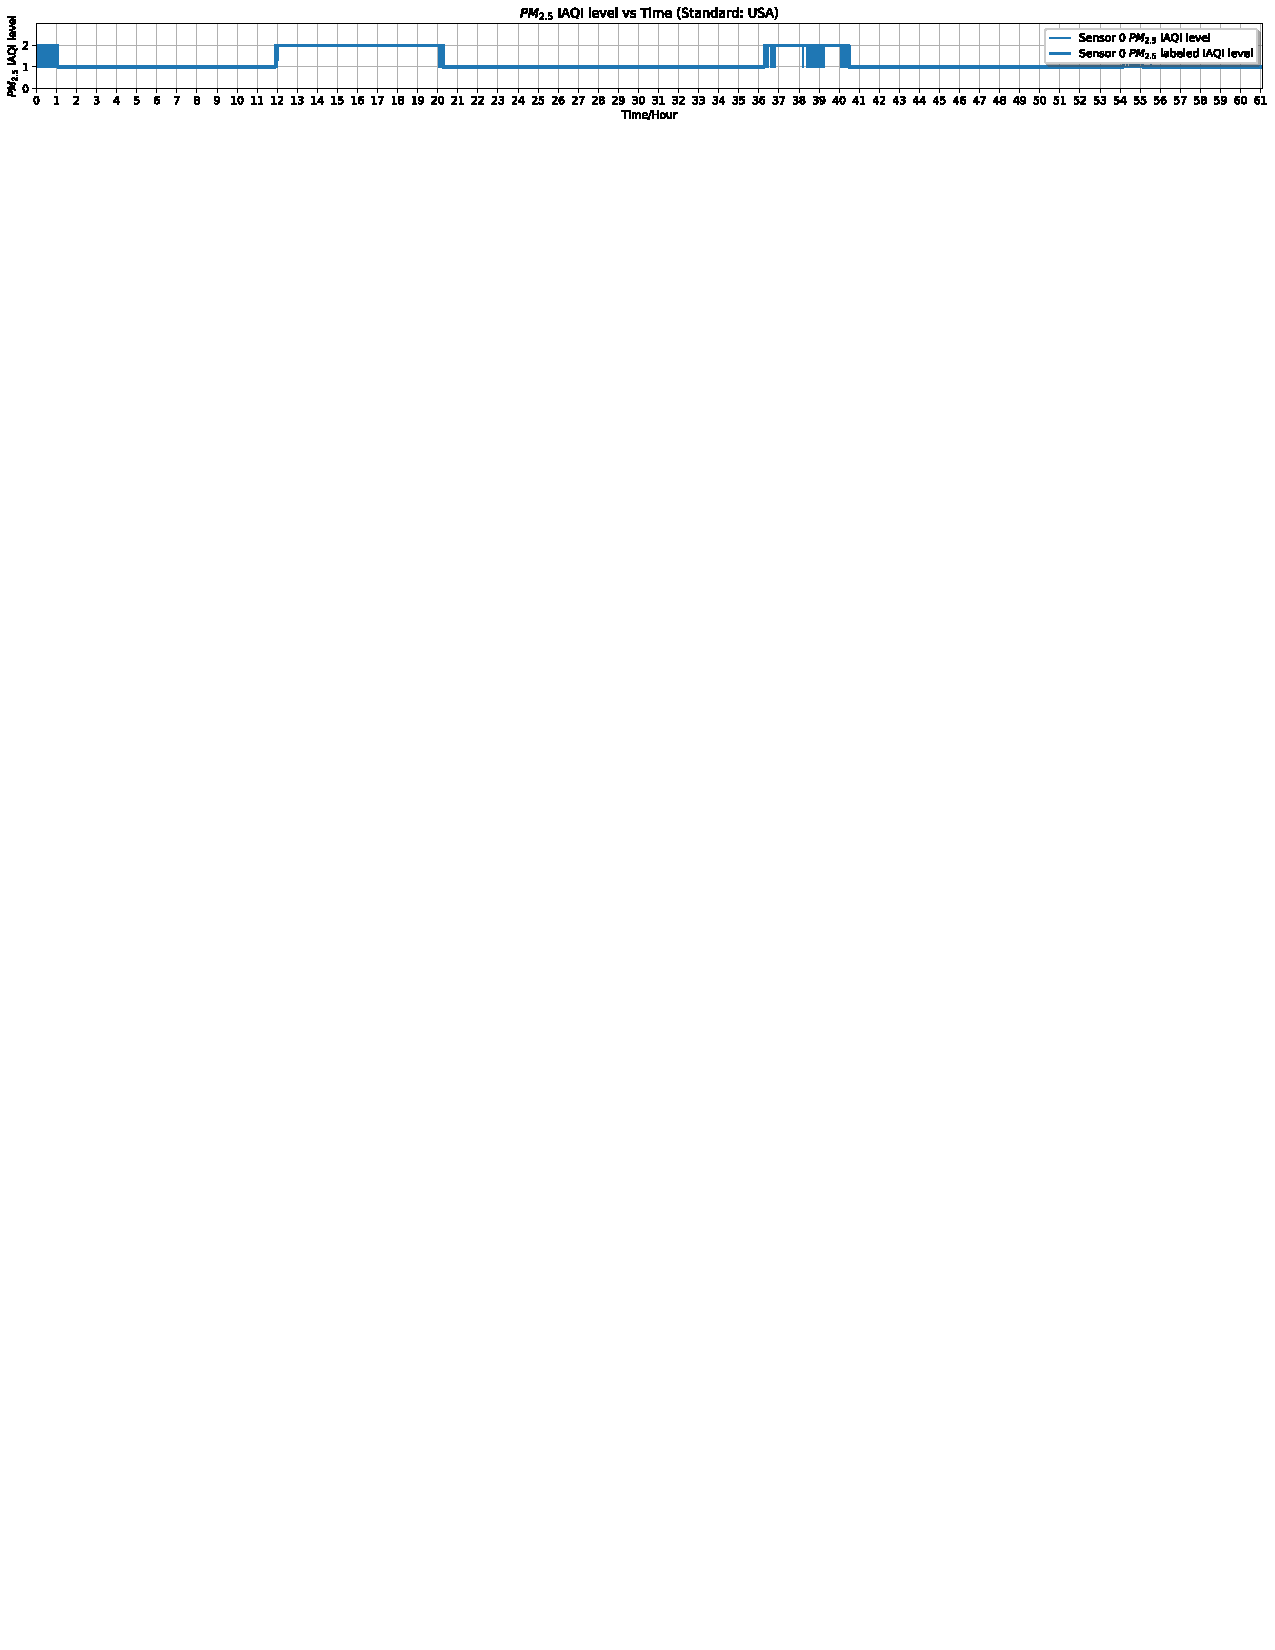
\includegraphics[width=\linewidth]{fig/labeled_iaqi_level/origin_and_labeled/pm25_0.png}
    \caption{Sensor 0's $PM_{2.5}$ origin and labeled IAQI level.}
    \label{fig:pm25_0_origin_and_labeled_level}
\end{figure}

\subsection{Data Polygonization}

To make use of the time elapse information, we did the same modeling as in \cite{rouet2017machine}. We did a similar transformation for the IAQI level plots (after labeling). Between two change points of the IAQI level, we transferred the level step-ups and downs into increasing and decreasing lines following the formula below:

\begin{equation}
    Level_t = (Level_{end}-Level_{begin}) / t-t_{begin}
\end{equation}

Dash lines in Figure \ref{fig:pm25_0_labeled_level} shows the results. These triangular lines will be label data for our later supervised learning regression problem.

\begin{figure}
    \centering
    \includegraphics[width=\linewidth]{fig/labeled_iaqi_level/pm25_0_labeled_iaqi_level.png}
    \caption{Sensor 0's labeled $PM_{2.5}$ IAQI level and its polygonization.}
    \label{fig:pm25_0_labeled_level}
\end{figure}

As the same with the modeling for acoustic data in \cite{rouet2017machine}, transferring step functions into linearly increasing/decreasing lines is a very useful method for preparing supervising data. These data contain linear time information. Thus the model can learn time variance knowledge between two change points of the IAQI level.

The level polygonal lines w.r.t. their manually labeled level curves can be written as equations with the form below:

\begin{equation}
    \label{formula:polygonal}
    L_i(t)=k_i*t+b_i, where t\in[t_i,t_{i+1}]
\end{equation}

Where $k_i$ is the slope of the curve, $t_i$ and $t_{i+1}$ start and end time point for every interval of the polygonal line. When $k_i>0$, the trend of the IAQI level is rising, and vice versa. The absolute value of $k_i$ is the approximate and potential changing speed of the IAQI level.

Thus, every polygonal line can be divided into several segments within time interval $t_i$ to $t_{i+1}$, and every segment estimates the 1-order approximate trend w.r.t. original IAQI level within the corresponding time interval. For the i-th segment, $k_i$ is $k_i =\frac{l_{i+1}-l_i}{t_{i+1}-t_i}$, where $l_{i+1}$ and $l_i$ are the original IAQI levels at end time $t_{i+1}$ and start time and $t_i$.

Finally, similar to B. Rouet-Leduc's work on earthquake predicting \cite{rouet2017machine} where the time-to-failures curve acts as y label, our experiments will take these polygonized IAQI level lines as the supervising data.

%!TEX program = xelatex
%!TEX root = ./thesis.tex
\chapter{Experiments}\label{chap:experiments}

% \yan{How about using the title ``Evaluations''?}
% No, thx.
% \yan{For grammar issues, do you mind using Grammarly \textit{https://app.grammarly.com/} to check your document? Our lab often uses it when writing English papers.}
% Yep, this whole thesis has already been revised on Grammarly.

The GreenEyes model is based on WaveNet and LSTM. Unlike computer vision models, which take 2D images as inputs, the GreenEyes model is trained on 1D sequential data arrays.

To build a data feeding pipeline, we built a slice data generator on the $PM_{2.5}$ IAQI data. Train data pairs as below are fed to the model:

\begin{equation}
\left\{
    \begin{array}{l}
    X_i=[D(t_i),D(t_{i+1}),...,D(t_{i+L-1})] \\
    y_i=P(t_{i+L})
    \end{array}
\right.
\end{equation}

% 实验目的是用window化的 IAQI 数据(注意是iaqi数据,不是原始pm数据)fit手动标注的 IAQI level

Where $D$ denotes the whole $PM_{2.5}$ IAQI data array, $P$ denotes the whole target function, i.e., the polygonized IAQI level we get in the last chapter. It is clear that our model takes a 1D array as input and outputs a scalar.

$L$ denotes the length of the slice when we sample sequences from the $PM_{2.5}$ IAQI data, and $t_i$, $t_{i+1}$ etc. are the discrete-time points. Note that to make the model to be \textbf{causal}, the target value $y_i$ in the train data pair is sampled at time point $t_{i+L}$, which is exactly next to the last time point in $X_i$.

In our experiment, as the total length of the $PM_{2.5}$ IAQI data is 219,989, setting different values for the length of the slice $L$ will firstly lead to variant input size for the GreenEyes model because the input size equals $L$, which will also make the number of training parameters larger or smaller. Secondly, as the length of the whole sequence data is limited, the larger $L$ is, the less the number of total train data is. Number of total train data is $(219,989-L+1)$.

We finally chose 7,200 as the length of the slice for the following reasons:
\begin{enumerate}
    \item 7,200 seconds equals 2 hours in the time axis, and we design the model to predict the next second's IAQI level by previous data within these 2 hours.
    \item The model's size (number of parameters, etc.) w.r.t. the input size of 7,200 is exactly appropriate both for learning and inferring.
\end{enumerate}

\section{Data Sampling and Splitting}

As described above, the number of total train data is $(219,989-L+1)$. When setting $L=7200$, it is 212,790, which is an enormous number when feeding the model. Hence, we introduced the sampling method and set stride when collecting train samples from the original data, and the size will be $\frac{\lfloor 219,989-L+1 \rfloor}{stride}+1$. 

Moreover, we split the data into a training set and validation set, with a validation ratio of 0.2. The number of training/validation samples varies when stride varies. Out experiments use 10, 5, 2 as stride's value and Table \ref{table:N_samples} illustrates the number of training/validation samples.

\begin{table}[!htbp]
    \centering
    \begin{tabular}{|l|l|l|l|l|}
    \hline
    $L$ (The length of the slice) & Stride & $N_{samples}$ & $N_{train}$ & $N_{val}$ \\ \hline
    7200 & 10 & 21280  & 17024  & 4256  \\ \hline
    7200 & 5  & 42559  & 34048  & 8511  \\ \hline
    7200 & 2  & 106396 & 85117  & 21279 \\ \hline
    \end{tabular}
    \caption{The relationship between different strides and number of samples.}
    \label{table:N_samples}
\end{table}

Figure \ref{fig:model_feeding_pipeline} shows the model feeding pipeline of our GreenEyes model during training.

\begin{figure}[!htbp]
    \centering
    \includegraphics[width=2.9in]{slides/data_slicing.pdf}
    \caption{Data feeding pipeline when training.}
    \label{fig:model_feeding_pipeline}
\end{figure}

\section{Sensor Data Augmentation}

As brought out before, we believe that with more data together, the model could learn better. Though these four data channels differ a little from each other, they approximately follow the same distribution. Hence, besides training the model on every single channel of \text{$PM_{2.5}$} data, we also \textbf{combined} all these channels' data together and fed it. The corresponding data is called \text{$PM_{2.5}$ (All)}.

\section{Experiments}
% 描述实验的组别,个数
As we sampled $PM_{2.5}$ data from 4 sensors, Sensor 0 to Sensor 3, so we have four channels of $PM_{2.5}$ IAQI data, and there are three different stride values. Finally, we have 12 experiments. Besides, we have a group of augmentation experiments in which all four sensors' data are fed to the model, yielding another three experiments.
% LR 配置
For each experiment, We optimized our GreenEyes model using Adam \cite{kingma2017adam} an initial learning rate of 0.0001, which is multiplied by 0.1 after 20 epochs. We trained our model to 100 epochs for each experiment.
% Loss 配置
We used mean squared error (MSE) as a loss metric and recorded mean absolute error (MAE). They are defined by equations below:

\begin{equation}
    MSE(p, y)=E((p_i-y_i)^2)
\end{equation}

\begin{equation}
    MAE(p, y)=E(|p_i-y_i|)
\end{equation}

Where $p$ is the prediction sequence and $y$ is the polygonized $PM_{2.5}$ IAQI sequence.

% four metrics, mean squared error (MSE), mean absolute percentage error (MAPE), mean squared logarithmic error (MSLE).

\subsection{Training and Validation} % 15 experiments

\subsubsection{Training Loss Curves}

Figure \ref{fig:training_mse} and Figure \ref{fig:val_mse} illustrate the training MSE curves and validation MSE curves respectively. It is observed that our system can fit the data well.
% \yan{Add a conclusion. } \yan{It is observed our system can xxx.}

% \yan{By the way, does your institution require inserting PDF figures?}

\begin{figure}[!htbp]
    \centering
    \begin{subfigure}[!htbp]{.45\textwidth}
        \centering
        \includegraphics[width=\textwidth]{fig/results/train_curves_stride_10.pdf}
        \caption{stride=10.}
        \label{fig:train_stride_10}
    \end{subfigure}
    \hfill
    \begin{subfigure}[!htbp]{.45\textwidth}
        \centering
        \includegraphics[width=\textwidth]{fig/results/train_curves_stride_5.pdf}
        \caption{stride=5.}
        \label{fig:train_stride_5}
    \end{subfigure}
    % \hfill
    \begin{subfigure}[!htbp]{.45\textwidth}
        \centering
        \includegraphics[width=\textwidth]{fig/results/train_curves_stride_2.pdf}
        \caption{stride=2.}
        \label{fig:train_stride_2}
    \end{subfigure}
\caption{Training MSE curves.}
\label{fig:training_mse}
\end{figure}

\begin{figure}[!htbp]
    \centering
    \begin{subfigure}[!htbp]{.45\textwidth}
        \centering
        \includegraphics[width=\textwidth]{fig/results/val_curves_stride_10.pdf}
        \caption{stride=10.}
        \label{fig:val_stride_10}
    \end{subfigure}
    \hfill
    \begin{subfigure}[!htbp]{.45\textwidth}
        \centering
        \includegraphics[width=\textwidth]{fig/results/val_curves_stride_5.pdf}
        \caption{stride=5.}
        \label{fig:val_stride_5}
    \end{subfigure}
    % \hfill
    \begin{subfigure}[!htbp]{.45\textwidth}
        \centering
        \includegraphics[width=\textwidth]{fig/results/val_curves_stride_2.pdf}
        \caption{stride=2.}
        \label{fig:val_stride_2}
    \end{subfigure}
\caption{Validation MSE curves.}
\label{fig:val_mse}
\end{figure}

% 讨论一个 Sensor,其它的放附录
% For Sensor 0, we fed the model with three different stride values. Figure
% the learning curves
% after the learning rate changes at the 20th epoch
% For more model training data, please refer to Appendix \ref{chapter:other_model_training_data}
% Figure \ref{fig:model_training_mse_mae_msle} shows the training process. We can infer that the model is already saturated after 100 epochs.

\subsubsection{Training Best Metrics}

As we used MSE as loss, i.e., the supervising metric, we extracted minimum train MSE and minimum validation MSE from all the training epochs. These best metric results reflect the model's fitting capability. They are all rounded to 4 decimals. 

% We also record other metrics such as MAE during training.

Table \ref{table:best_metrics} lists each experiment's final best metrics during training.

\begin{table}[!htbp]
    \centering
    \begin{tabular}{|c|c|c|c|c|}
        \hline\hline
        Data & Stride & Minimum train MSE & Minimum validation MSE & ratio \\\hline
        \multirow{3}{*}{\text{$PM_{2.5}$(0)}} & 10 & 0.0223 & 0.0234 & 0.96 \\ \cline{2-5} 
                                        & 5 & 0.0034 & 0.0114 & 0.30 \\ \cline{2-5} 
                                        & 2 & \textbf{\textit{0.0006}} & \textbf{\textit{0.0035}} & 0.16 \\ \hline
        \multirow{3}{*}{\text{$PM_{2.5}$(1)}} & 10 & 0.0486 & 0.0510 & 0.95 \\ \cline{2-5} 
                                        & 5 & 0.0058 & 0.0142 & 0.41 \\ \cline{2-5} 
                                        & 2 & \textbf{\textit{0.0006}} & \textbf{\textit{0.0036}} & 0.17 \\ \hline
        \multirow{3}{*}{\text{$PM_{2.5}$(2)}} & 10 & 0.0171 & 0.0187 & 0.92 \\ \cline{2-5} 
                                        & 5 & 0.0024 & 0.0092 & 0.27 \\ \cline{2-5} 
                                        & 2 & \textbf{\textit{0.0012}} & \textbf{\textit{0.0066}} & 0.19 \\ \hline
        \multirow{3}{*}{\text{$PM_{2.5}$(3)}} & 10 & 0.0509 & 0.0468 & 1.09 \\ \cline{2-5} 
                                        & 5 & 0.0074 & 0.0167 & 0.44 \\ \cline{2-5} 
                                        & 2 & \textbf{\textit{0.0010}} & \textbf{\textit{0.0068}} & 0.15 \\ \hline
        \multirow{3}{*}{\text{$PM_{2.5}$(All)}} & 10 & 0.0068 & 0.0103 & 0.66 \\ \cline{2-5} 
                                        & 5 & 0.0014 & 0.0022 & 0.67 \\ \cline{2-5} 
                                        & 2 & \textbf{0.0007} & \textbf{0.0009} & 0.77 \\
        \hline
        \hline
    \end{tabular}
    \caption{Experiments' final best metrics.}
    \label{table:best_metrics}
\end{table}

We also define a generalization coefficient ratio as the equation below to measure the model's generalization capability during certain experiments. The larger the ratio,  the better the generalization capability is. The ratio results are rounded to 2 decimals.

\begin{equation}
    ratio=\frac{min(train\ MSE)}{min(validation\ MSE)}
\end{equation}

\subsection{Model Evaluation}

% Evaluation curves
\begin{figure}
    \centering
    \includegraphics[width=\linewidth]{fig/model_eval_pm25_0_stride_10.png}
    \caption{Evaluation of the GreenEyes model (\text{$PM_{2.5} (0)$}, stride=10).}
    \label{fig:model_eval_pm25_0_stride_10}
\end{figure}

As earthquake prediction aims to fit the model and learn time-series information, i.e., the triangular lines in coordination with the acoustic data, our model also fits the level lines regarding their air pollutant concentration data. Figure \ref{fig:model_eval_pm25_0_stride_10} proves that the model fits the labeled IAQI level lines well, except that its predictions differ from the ground truth a little on some parts of the lines, and especially on the turning corners of the piecewise linear function.

% Test results table here.
To quantify the testing results of our model by different parameters, we tested it on the whole $PM_{2.5}$ sequence by setting stride as 1, which is different from the training config. As stride is set to 1, the slice window will move one point after another. Hence, the model can make the inference on the whole source sensor data. When the stride is set a 10, 5, and 2 for different training data sampling configs, these sampled data slices form a subset of the sliced data when the stride is set to 1.

We performed the tests using two metrics, mean square error (MSE) and mean absolute error (MAE).

And we test all models trained under different stride parameters and on every channel of $PM_{2.5}$ data. Table \ref{table:test_mse_mae} lists the statistics of our tests. Digit in the brackets is the channel number. "All" means the model is trained by all channels together. All result values of MSE have rounded four decimals, and all MAE values are rounded to 2 decimals.

\begin{table}[!htbp]
    \centering
    \begin{tabular}{|c|c|c|c|}
        \hline\hline
        Data & Stride & MSE & MAE \\\hline
        \multirow{3}{*}{\text{$PM_{2.5}$(0)}} & 10 & 0.0266 & 0.13 \\ \cline{2-4} 
                                        & 5 & 0.0144 & 0.11 \\ \cline{2-4} 
                                        & 2 & \textbf{\textit{0.0037}} & \textbf{\textit{0.05}} \\ \hline
        \multirow{3}{*}{\text{$PM_{2.5}$(1)}} & 10 & 0.0517 & 0.18 \\ \cline{2-4} 
                                        & 5 & 0.0113 & 0.10 \\ \cline{2-4} 
                                        & 2 & \textbf{\textit{0.0036}} & \textbf{\textit{0.05}} \\ \hline
        \multirow{3}{*}{\text{$PM_{2.5}$(2)}} & 10 & 0.0188 & 0.11 \\ \cline{2-4} 
                                        & 5 & 0.0092 & 0.09 \\ \cline{2-4} 
                                        & 2 & \textbf{\textit{0.0069}} & \textbf{\textit{0.07}} \\ \hline
        \multirow{3}{*}{\text{$PM_{2.5}$(3)}} & 10 & 0.0501 & 0.16 \\ \cline{2-4} 
                                        & 5 & 0.0108 & 0.09 \\ \cline{2-4} 
                                        & 2 & \textbf{\textit{0.0070}} & \textbf{\textit{0.07}} \\ \hline
        \multirow{3}{*}{\text{$PM_{2.5}$(All)}} & 10 & 0.0118 & 0.09 \\ \cline{2-4} 
                                        & 5 & 0.0026 & 0.04 \\ \cline{2-4} 
                                        & 2 & \textbf{0.0010} & \textbf{0.02} \\ \hline
        \hline
        \hline

    \end{tabular}
    \caption{Test MSE and MAE under different strides.}
    \label{table:test_mse_mae}
\end{table}

The data on the table shows that for each channel of $PM_{2.5}$ data, the smaller the stride parameter is, the less the MSE and MAE are, which means the model can fit the target better. This is reasonable and consistent with our intuition.

Meanwhile, when put all channels' data together and feed the model, it can learn the best result.

Figure \ref{fig:test_mse} and Figure \ref{fig:test_mae} respectively present the test MSE and MAE results by bar plots. The plots are divided into three stride groups, which's stride is 10, 5, 2. Results from the different data channels (or all channels of the data) but sharing the same stride join into the same group for comparisons.

\begin{figure}[!htbp]
    \centering
    \begin{subfigure}[!htbp]{.45\textwidth}
        \centering
        \includegraphics[width=\textwidth]{fig/results/test_mse.pdf}
        \caption{Test MSE.}
        \label{fig:test_mse}
    \end{subfigure}
    \begin{subfigure}[!htbp]{.45\textwidth}
        \centering
        \includegraphics[width=\textwidth]{fig/results/test_mae.pdf}
        \caption{Test MAE.}
        \label{fig:test_mae}
    \end{subfigure}
    \caption{Test MSE and MAE.}
    \label{fig:test_mse_mae}
\end{figure}

\subsection{Results Analyses}

From the results table and bar plots, we could draw at least two useful and meaningful conclusions. Firstly, for each kind of data, whichever $PM_{2.5}$ (i) or $PM_{2.5}$ (All), when the stride parameter decreases, the model can outcome better results.

Secondly, in each stride group, $PM_{2.5}$ (All)'s performance surpasses every single channel of $PM_{2.5}$ data, w.r.t. both MSE and MAE. And when the stride is 5 or 2, this conclusion is more significant.

The first conclusion is obvious. As Table \ref{table:N_samples} shows, the smaller the stride is, the number of training samples gets larger. More data will result in a better model's fitting performance. However, while we want the model to predict and fit more precisely, we don't want to sample sliced data from original data flow too frequently (set the stride too small). The model's capability is reflected by its relevant fitting results (MSE, MAE, etc.), while a rather less frequent sampling is configured (e.g., set stride to 10, not 2).

For our GreenEyes model, the evaluation curve in Figure \ref{fig:model_eval_pm25_0_stride_10} shows its fitting capability, as stride 10 is already enough.

During application, we could trade off on this stride parameter to balance the model's performance and the computation costs.

%!TEX program = xelatex
%!TEX root = ../thesis.tex

\chapter{Discussion}\label{chap:discussion}

% \yan{Do you think it is better to divide this section into two subsections: limitations, future research directions?}
% Thx, but no. Boss let me to write them into one single chapter.
We proposed the GreenEyes model to solve the time series fitting problems in air pollution evaluation. Compared with related works such as GNN, our model's architecture is simpler and easier to be distributed. Its components are relatively basic, making it easier to do feature analyzing works and more possibly interpretable. Our model inherits effective but not complex components such as residual connections and 1D dilated convolution from WaveNet. By stacking WaveNet layers, our model becomes modulized, and its data throughput capability has been enhanced.

Just as we introduced by related work, Arduino \cite{okokpujie2018smart}, ARM \cite{ailing2017design} could also be used for IoT design and data collection. We have designed an ARM platform to collect the air pollution data, which can also send data to PC. However, we retrieve data through a USB connection between the sensors and the computer for our current time series fitting work. For wireless data transmission demands such as BLE and WiFi, the ARM platform is optional in our work design.

As for the engineering price, four sensors in our experiments cost only about 400 RMB. For model training, we did our experiments on a single-channel 1080 Ti GPU. When hyper-parameter stride is set to 10, it costs about 1 hour to train the model on one channel of the sensor's data for 100 epochs, which is enough to get it saturated. When stride is set to 5, it costs about 2 hours, and 6 hours for stride is 2.

In this thesis, we placed all the four sensors at the same place to validate the sensors' reliability and stability. In another way, we also proved the idea of data augmentation, which means the more the data, the better performance the model could yield. However, these data from 4 sensors are pretty homogeneous compared with those from scenarios where sensors are distributed in various places. During the same time, many works such as GNN \cite{wu2020connecting} conclude feasible methods to do correlation analysis between data from multi-sources.

Hence, firstly, correlation analysis could be done through these methods, without regard to whether we put our sensors at the same place or distribute them at different spots. This method could be used to better validate the sensors' reliability. Secondly, for the distributed cases, if the correlation information is found, works related to air pollution sensor network designing could be progressed, such as data fusion for multi types of sensors and air pollution spatial interpolation. Spatial interpolation problems are also essential, especially for path planning tasks in scenarios such as urban transportation planning.

When it comes back to time series forecasting problems, a pity shortcoming of this thesis is that we haven't collected enough data for the forecasting problem, so we just did the fitting work. Our sensors could collect more valid data for training our model. Data could also be collected from all kinds of data platforms, such as websites. If the quantity of the collected data is large enough and their effectiveness and reliability are ensure, we could conduct more experiments and research in the future.
% Potential application
Finally, the intention of our work gives considerations to both academic research and industrial application. Nowadays, neural network inference algorithms could be distributed on mobile phones due to the development of mobile computational platforms. For instance, TensorFlow provides a tool package called TensorFlow Lite. If our model is transferred into mobile phones, given a smart sensor unit that is able to transmit data, the phones could do the inference and prediction without a PC. I believe this is a practical solution for those AIoT users.

%!TEX program = xelatex
%!TEX root = ./thesis.tex
\chapter{Conclusion}

The WaveNet model designed for audio data processing is generalizable and suitable for regression such as time series forecasting. Our work successfully put it into usage for the IAQI level fitting problem. It shows that our GreenEyes model based on WaveNet has strong data fitting capability as the lengths of the input data sequences can be very large.

The GreenEyes model fits the processed train data well and predicts well on coordinated validation and test data. Both the MSE metric and MAE metric could converge into a small value.

It is also found that, when trained with more channels of sensor data, the model can perform well. In somehow, this trick could be regarded as sensor data augmentation.

Our innovative method that humans manually label the IAQI level is useful. It creates an appropriated target label function that the model can learn. Also, based on the labeling tricks, the problem that the predictions on the IAQI level will fluctuate near the thresholds is quite reduced. Furthermore, it comes from a real scenario when users interact with this machine learning product and system.

It is well tested that our GreenEyes AIoT system is dependable and has versatile applications. An app has been developed half the way to monitor the IAQI data in real-time when sensors are connected. GreenEyes' deep learning model can also be installed on the mobile and predict the IAQI level.

%%%%%%%%%%%%%%%%%%%%%%%%%%%%%%%%%%%%%%%%%%%%%%%%%%%%%%%%%%%%%%%%%%%%%%%%%
%                                                                       %
%      9) BIBLIOGRAPHY                                                  %
%                                                                       %
% This example uses bibtex to generate the required Bibliography. Refer %
% to the % the file ustthesis_test.bib for the entries of the           %
% Bibliography. Note that only the cited entries are printed.           %
%                                                                       %
% If BibTeX is not used to typeset the bibliography, replace the        %
% following line with the \begin{thebibliography} and \end{bibliography}%
% commands (the "thebibliography" environment) to process the           %
% Bibliography.                                                         %
%                                                                       %
%%%%%%%%%%%%%%%%%%%%%%%%%%%%%%%%%%%%%%%%%%%%%%%%%%%%%%%%%%%%%%%%%%%%%%%%%

%%%%%%%%%%%%%%%%%%%%%%%%%%%%%%%%%%%%%%%%%%%%%%%%%%%%%%%%%%%%%%%%%%%%%%%%%
%                                                                       %
% The recommended bibliography style is the IEEE bibliography style.    %
% "ustbib" defines the IEEE bibliography standard with the added        %
% ability of sorting the items by name of author.                       %
%                                                                       %
% If you are not using BibTeX to process your Bibliography, comment out %
% the following line.                                                   %
%                                                                       %
%%%%%%%%%%%%%%%%%%%%%%%%%%%%%%%%%%%%%%%%%%%%%%%%%%%%%%%%%%%%%%%%%%%%%%%%%

\bibliographystyle{plain}
\bibliography{citations/citations}
% Please run "bibtex ustthesis_test" before the bibliography can be
% included.

%%%%%%%%%%%%%%%%%%%%%%%%%%%%%%%%%%%%%%%%%%%%%%%%%%%%%%%%%%%%%%%%%%%%%%%%%
%                                                                       %
%     10) APPENDIX (If Any)                                             %
%                                                                       %
% \appendix command marks the beginning of the APPENDIX part of the     %
% Thesis. The usual \chapter command is used for the different chapters %
% of the Appendix.                                                      %
%                                                                       %
%%%%%%%%%%%%%%%%%%%%%%%%%%%%%%%%%%%%%%%%%%%%%%%%%%%%%%%%%%%%%%%%%%%%%%%%%

%!TEX program = xelatex
%!TEX root = ./thesis.tex
\appendix

\chapter{Miscellaneous IAQI Standards}\label{chapter:IAQI_standards}

This appendix section lists a complete data preprocessing results

It uses the same way to map concentration data into IAQI, and finally calculates AQI, the only different is the thresholds. Both USA and China use the maximum IAQI to represent final AQI.

According to Technical Regulation on Ambient Air Quality Index (on trial) \cite{regulation2012} release by former Ministry of Environmental Protection of the People's Republic of China, IAQI (individual air quality index) and AQI (air quality index) should be calculated by the following equations:

\begin{equation}
    IAQI_p = \frac{IAQI_{Hi}-IAQI_{Lo}}{BP_{Hi}-BP_{Lo}}(C_p-BP_{Lo})+IAQI_{Lo}
\end{equation}

or equivalently:

\begin{equation}
    \label{formula:IAQI_appendix1}
    IAQI_p = \frac{C_p-BP_{Lo}}{BP_{Hi}-BP_{Lo}}(IAQI_{Hi}-IAQI_{Lo})+IAQI_{Lo}
\end{equation}

In formula \ref{formula:IAQI_appendix1}, $C_p$ is the concentration value for certain category like $PM_{2.5}$; $BP_{Hi}$ and $BP_{Lo}$ are high threshold/low threshold near $C_p$, respectively; $IAQI_{Hi}$ and $IAQI_{Lo}$ are high threshold/low threshold $C_p$, respectively.

Then calculate AQI by making use of the maximum of these individual IAQI values \ref{appendix:formula:AQI}:

\begin{equation}
    \label{appendix:formula:AQI}
    AQI = \max\{IAQI_1,IAQI_2,IAQI_3,...,IAQI_n\}
\end{equation}

For each pollutant category, concentration value will firstly all be mapped into the IAQI value according to its corresponding thresholds in the thresholds table \ref{table:IAQI-thresholds}.

The regulation \cite{regulation2012} determines concentration value thresholds for pollutant categories such as $SO_2$, $NO_2$, $CO$, $PM_{2.5}$, $PM_{10}$ and $O_3$. For one-hour average value and 24-hour average value, thresholds are determined differently, for $SO_2$, $NO_2$, $CO$. Note that the thresholds for $PM_{2.5}$ and $PM_{10}$ concentration value are defined by their 24-hour average, this means the method of calculating IAQI for a single day. However, it doesn't matter when we uses these thresholds for realtime (1 Hz) $PM_{2.5}$ and $PM_{10}$ concentration data. Table \ref{table:IAQI-thresholds} shows the $PM_{2.5}$ and $PM_{10}$ data-IAQI mapping relationship. Followed by data we could collect in our AIoT system, we only consider $PM_{2.5}$ and $PM_{10}$ data.

\begin{table}[!htbp]
    \centering
    \caption{Concentration thresholds of IAQI with regard to pollutant categories, China}
    \label{table:IAQI-thresholds}
    \begin{tabular}{|l|l|l|}
    \hline
    IAQI & $PM_{2.5}$ ($\mu g/m^3$) & $PM_{10}$ ($\mu g/m^3$) \\ \hline
    0    & 0   & 0   \\ \hline
    50   & 35  & 0   \\ \hline
    100  & 75  & 150 \\ \hline
    150  & 115 & 250 \\ \hline
    200  & 150 & 350 \\ \hline
    300  & 250 & 420 \\ \hline
    400  & 350 & 500 \\ \hline
    500  & 500 & 600 \\ \hline
    \end{tabular}
\end{table}

Use the formula and table above, we can plot in Figure \ref{fig:iaqi} the value-IAQI mapping curve for both $PM_{2.5}$ and $PM_{10}$. This is a visualization for the air pollutant concentration and its IAQI. For each category, data vary from 0 to 800, linearly.

\begin{figure}[!htbp]
    \centering
    \includegraphics[width=0.7\linewidth]{fig/iqai.pdf}
    \caption{IAQI curve of $PM_{2.5}$ (orange line) and $PM_{10}$ (green line) data.}
    \label{fig:iaqi}
\end{figure}

For data we collected, following the the IAQI thresholds table, each data of a pollutant category are mapped into IAQI values and have six levels, level 1 to 6. In USA's Technical Assistance Document \cite{daq2018} level 1 to 6 of the air quality index is represented by color \colorbox{green}{green}, \colorbox{yellow}{yellow}, \colorbox{orange}{orange}, \colorbox{red}{red}, \colorbox{purple}{purple} and \colorbox{maroon}{maroon}, respectively. We mapped our $PM_{2.5}$ and $PM_{10}$ data into IAQI respectively, as Figure \ref{fig/pm25_all_iaqi} and Figure \ref{fig/pm10_all_iaqi} shows.

\begin{figure}[!htbp]
    \begin{center}
    \includegraphics[width=\linewidth]{fig/iaqi/pm25_all_iaqi.png}
    \end{center}
    \caption{All $PM_{2.5}$ IAQI data.}
    \label{fig/pm25_all_iaqi}
\end{figure}

\begin{figure}[!htbp]
    \begin{center}
    \includegraphics[width=\linewidth]{fig/iaqi/pm10_all_iaqi.png}
    \end{center}
    \caption{All $PM_{10}$ IAQI data.}
    \label{fig/pm10_all_iaqi}
\end{figure}

\section{Other IAQI Calculation Method}
The air pollutant concentration thresholds are different in USA's Technical Assistance Document \cite{daq2018}, see Table \ref{table:IAQI-thresholds-USA}.

\begin{table}[!htbp]
    \centering
    \caption{Concentration thresholds of IAQI with regard to pollutant categories, USA}
    \label{table:IAQI-thresholds-USA}
    \begin{tabular}{|l|l|l|}
    \hline
    IAQI & $PM_{2.5}$ ($\mu g/m^3$) & $PM_{10}$ ($\mu g/m^3$) \\ \hline
    0    & 0     & 0   \\ \hline
    50   & 12.1  & 55  \\ \hline
    100  & 35.5  & 155 \\ \hline
    150  & 55.5  & 255 \\ \hline
    200  & 150.5 & 355 \\ \hline
    300  & 250.5 & 425 \\ \hline
    500  & 500.4 & 604 \\ \hline
    \end{tabular}
\end{table}

It uses the same way to map concentration data into IAQI, and finally calculates AQI, the only different is the thresholds. Both USA and China use the maximum IAQI to represent final AQI. As for Hong Kong's method for IAQI and AQI calculation, they use integer AQHI(Air Quality Health Index) and map it into five health risk levels. AQHI uses the \textbf{sum} of the sum of the percentage added health risk (\%AR) with regard to the 3-hour moving average concentrations belonging to four criteria of air pollutants: ozone ($O_3$), nitrogen dioxide ($NO_2$), sulphur dioxide ($SO_2$), and particulate matter (PM) \cite{aqhi2018}.

The calculation uses weighting and exponent, for example:

\begin{equation}
    \%AR(PM_{2.5}) = (e^{(\beta(PM_{2.5})\times C(PM_{2.5}))} – 1) \times 100\%
\end{equation}

where $\beta(PM_{2.5})$ is the added health risk factor for $PM_{2.5}$ and $\beta(PM_{2.5})=0.0002180567$. It is a regression coefficient technically.


\chapter{Other Data Preprocessing Results}\label{chapter:other_data_preprocessing_results}

This appendix section lists the complete data preprocessing results.

Figure \ref{fig:appendix:all_pm25_iaqi_level} shows

\begin{figure}[!htbp]
    \begin{center}
        \includegraphics[width=\linewidth]{fig/iaqi_level/pm25_0_iaqi_level_dpi1200.png}
    \end{center}
    \begin{center}
        \includegraphics[width=\linewidth]{fig/iaqi_level/pm25_1_iaqi_level_dpi1200.png}
    \end{center}
    \begin{center}
        \includegraphics[width=\linewidth]{fig/iaqi_level/pm25_2_iaqi_level_dpi1200.png}
    \end{center}
    \begin{center}
        \includegraphics[width=\linewidth]{fig/iaqi_level/pm25_3_iaqi_level_dpi1200.png}
    \end{center}
    \caption{All $PM_{2.5}$ IAQI level.}
    \label{fig:appendix:all_pm25_iaqi_level}
\end{figure}

Figure \ref{fig:appendix:all_pm25_iaqi_level_and_labeled} shows the origin IAQI level and labeled IAQI level in same figures. Origin IAQI level and labeled IAQI level are plotted with different linewidth. For each subfigure, the bolder line is the labeled IAQI level, and is wrapping the orgin IAQI curve, with contrast to the origin IAQI level.

\begin{figure}[!htbp]
    \begin{center}
        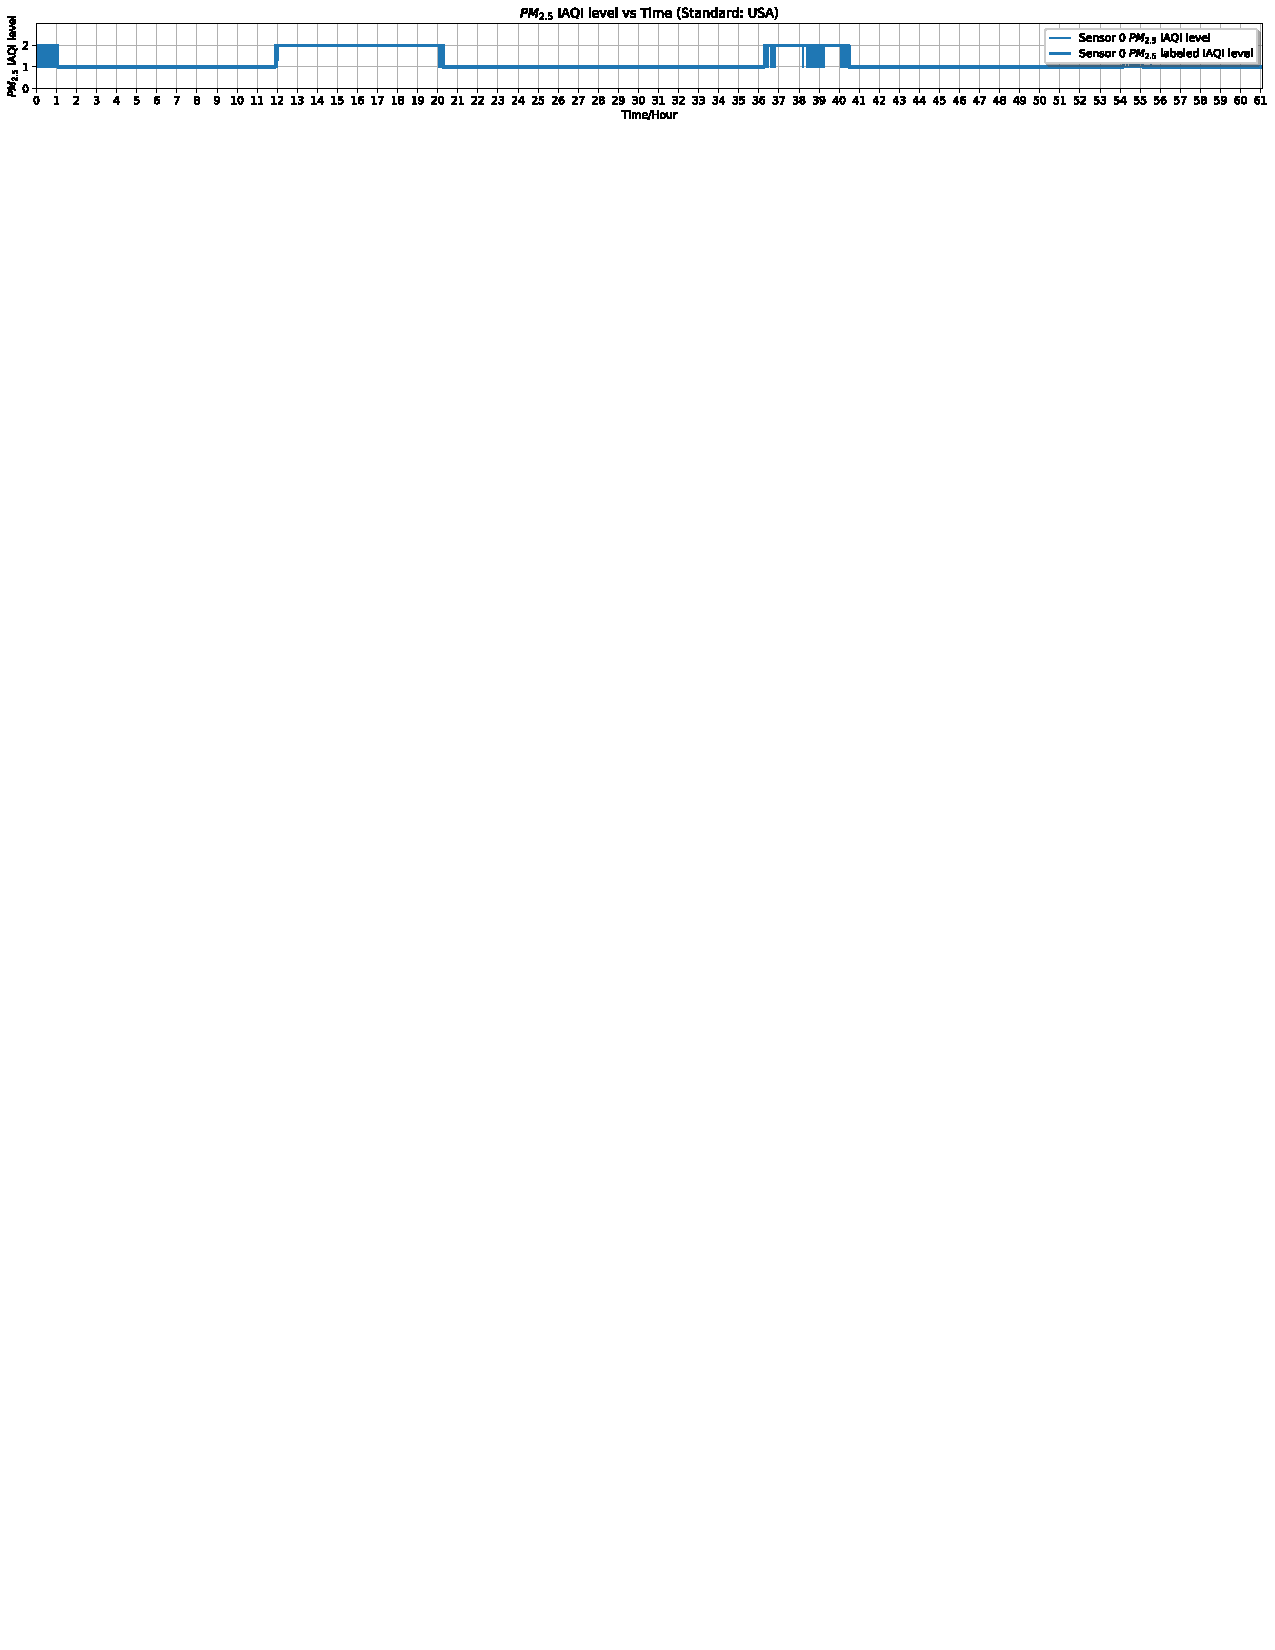
\includegraphics[width=\linewidth]{fig/labeled_iaqi_level/origin_and_labeled/pm25_0.png}
    \end{center}
    \begin{center}
        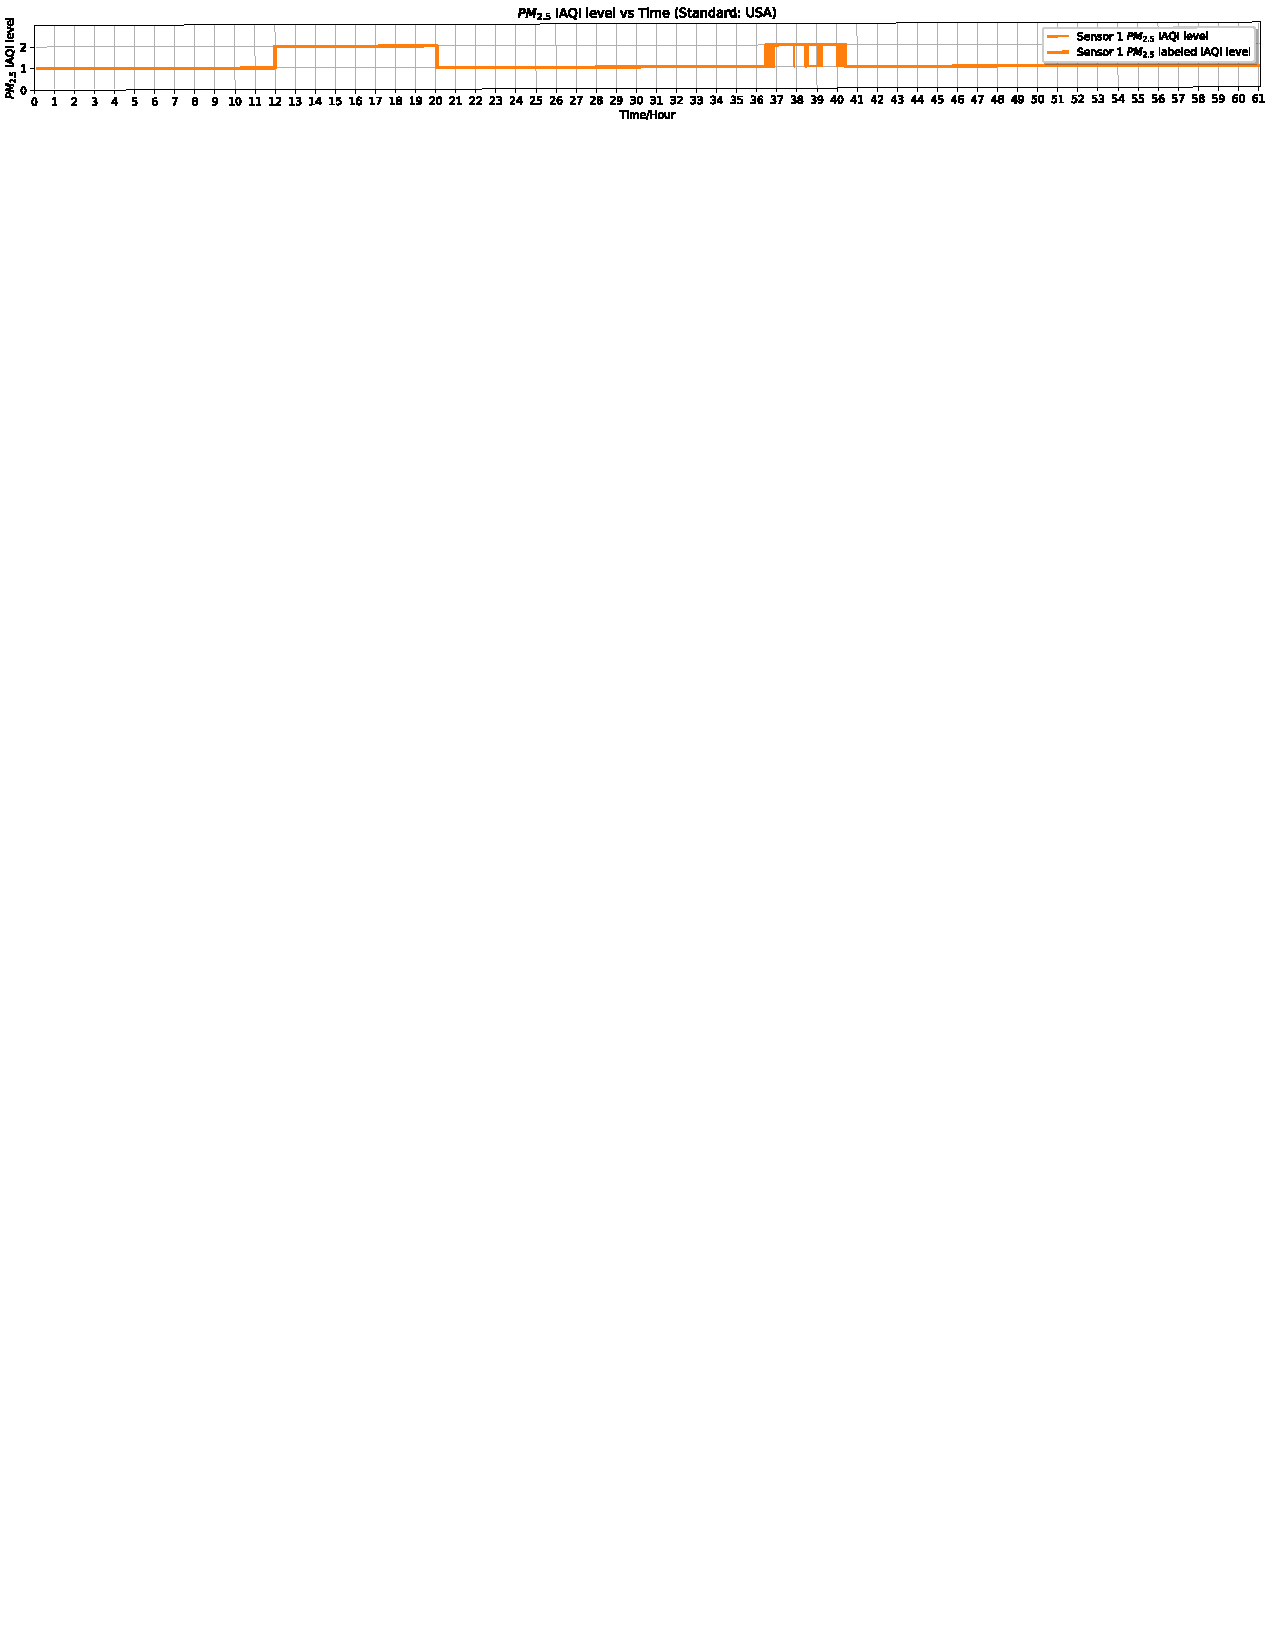
\includegraphics[width=\linewidth]{fig/labeled_iaqi_level/origin_and_labeled/pm25_1.png}
    \end{center}
    \begin{center}
        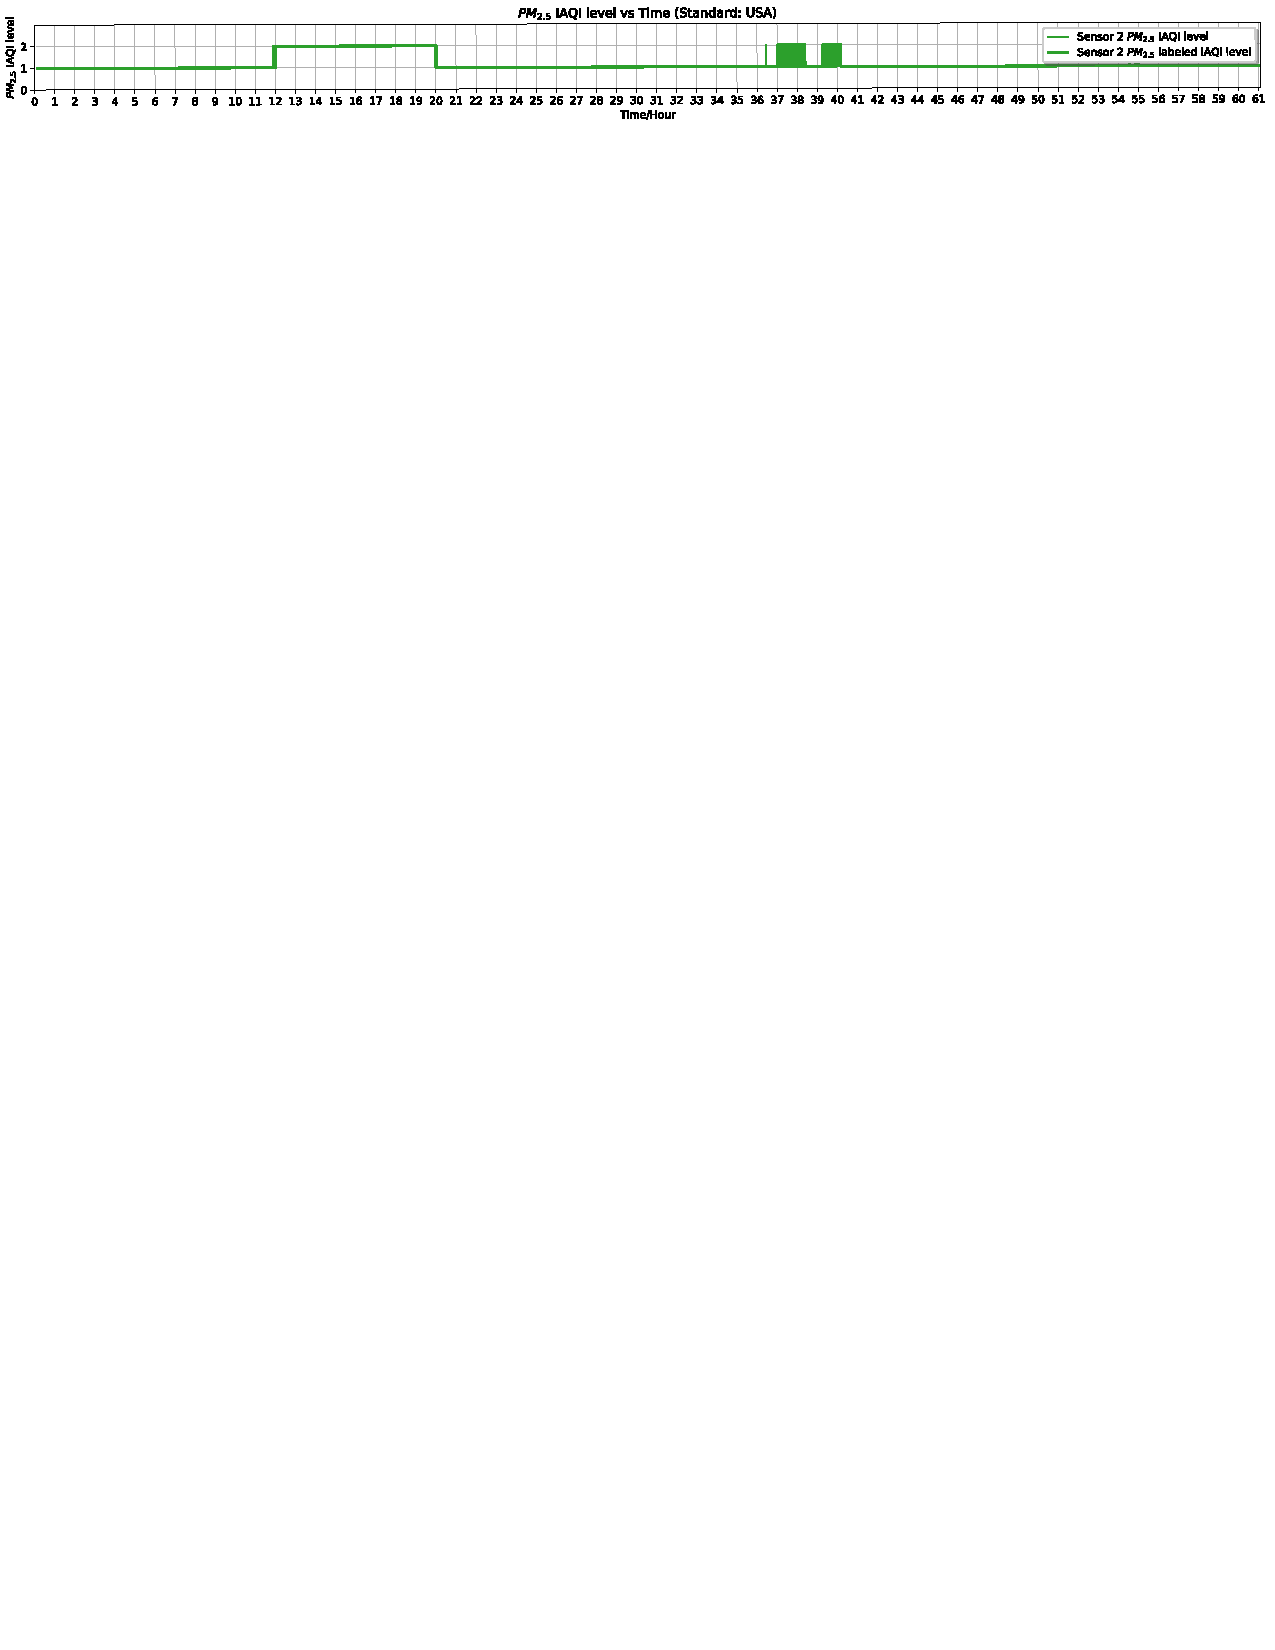
\includegraphics[width=\linewidth]{fig/labeled_iaqi_level/origin_and_labeled/pm25_2.png}
    \end{center}
    \begin{center}
        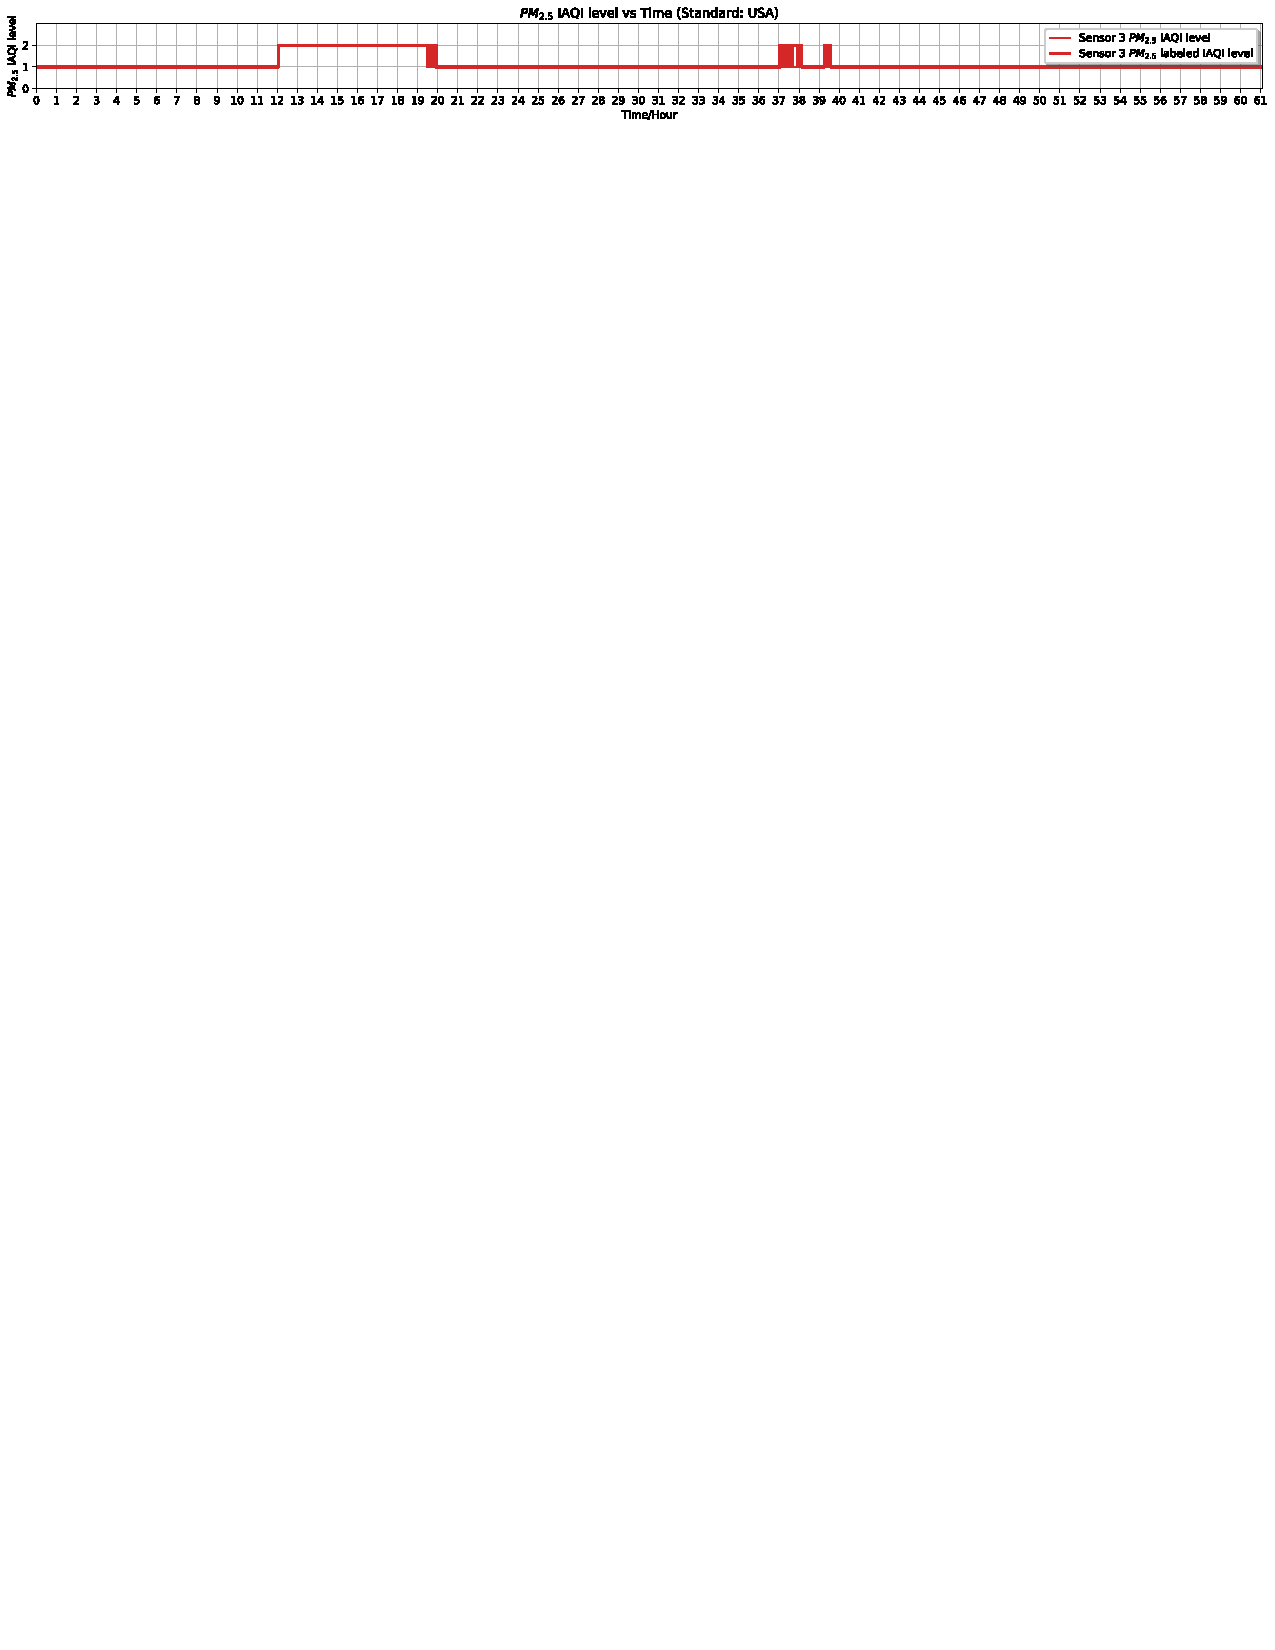
\includegraphics[width=\linewidth]{fig/labeled_iaqi_level/origin_and_labeled/pm25_3.png}
    \end{center}
    \caption{All labeled $PM_{2.5}$ IAQI level.}
    \label{fig:appendix:all_pm25_iaqi_level_and_labeled}
\end{figure}

Figure \ref{fig:appendix:all_pm25_polygonalized_iaqi_level} shows the results of yielding all polygonalized IAQI level lines from the labeled IAQI level.

\begin{figure}[!htbp]
    \begin{center}
        \includegraphics[width=\linewidth]{fig/labeled_iaqi_level/pm25_0_labeled_iaqi_level.png}
    \end{center}
    \begin{center}
        \includegraphics[width=\linewidth]{fig/labeled_iaqi_level/pm25_1_labeled_iaqi_level.png}
    \end{center}
    \begin{center}
        \includegraphics[width=\linewidth]{fig/labeled_iaqi_level/pm25_2_labeled_iaqi_level.png}
    \end{center}
    \begin{center}
        \includegraphics[width=\linewidth]{fig/labeled_iaqi_level/pm25_3_labeled_iaqi_level.png}
    \end{center}
    \caption{All polygonalized $PM_{2.5}$ IAQI level.}
    \label{fig:appendix:all_pm25_polygonalized_iaqi_level}
\end{figure}

% 多余的
% \chapter{Other Model Training Data}\label{chapter:other_model_training_data}


%%%%%%%%%%%%%%%%%%%%%%%%%%%%%%%%%%%%%%%%%%%%%%%%%%%%%%%%%%%%%%%%%%%%%%%%%
%                                                                       %
%     11) BIOGRAPHY (Optional)                                          %
%                                                                       %
% \biography and \endbiography are used to define the optional          %
% Biography of the author of the Thesis.                                %
%                                                                       %
%%%%%%%%%%%%%%%%%%%%%%%%%%%%%%%%%%%%%%%%%%%%%%%%%%%%%%%%%%%%%%%%%%%%%%%%%

% \biography
% The biography of the student is ALSO optional.
% \endbiography

\end{document}
